\documentclass[12pt, a4paper, oneside]{book}
\usepackage[hidelinks]{hyperref}
\usepackage[english]{babel}
\usepackage{epsfig}
\usepackage{epstopdf}
\usepackage[chapter]{algorithm}
\usepackage{algorithmic}
\usepackage{listings}
\usepackage{amsmath}
\usepackage{dirtytalk}
\usepackage{amssymb}
\usepackage{float}
\usepackage{graphicx}
\usepackage{multirow}
\usepackage{color}
\usepackage{url}
\usepackage[utf8]{inputenc}
\usepackage[T1]{fontenc}
\usepackage{setspace}
\usepackage{tabularx}
\usepackage{tabu}
\usepackage{pbox}
\usepackage{textcomp}
\usepackage{caption}
\usepackage{subfig}
\usepackage{natbib}
% \usepackage{nopageno}


\setstretch{1.5}
%\renewcommand\baselinestretch{1.5} % riadkovanie jeden a pol

\newcommand\mftitle{Algorithm development for the segmentation of astronomical images with unique features}
\newcommand\mfthesistype{Diplomová práca}
\newcommand\mfauthor{Bc. Viktor Nagy}
\newcommand\mfadvisor{Mgr. Jiří Šilha, PhD.}
\newcommand\mfconsultant{prof. RNDr. Roman Ďurikovič, PhD.}
\newcommand\mfplacedate{Bratislava, 2019}
\newcommand\mfuniversity{UNIVERZITA KOMENSKÉHO V BRATISLAVE}
\newcommand\mffaculty{FAKULTA MATEMATIKY, FYZIKY A INFORMATIKY}
\newcommand{\sub}[1]{$_{\text{#1}}$}
\newcommand{\reference}[1]{č.~\ref{#1}}
\newcommand{\imageHeight}{150px}
\pagestyle{empty}

\ifx\pdfoutput\undefined\relax\else\pdfinfo{ /Title (mftitle) /Author (\mfauthor) /Creator (PDFLaTeX) } \fi

\begin{document}

\frontmatter

% \thispagestyle{empty}

\noindent
\begin{minipage}{\textwidth}
\begin{center}
\textbf{\mfuniversity \\
\mffaculty}
\end{center}
\end{minipage}

\vfill
\begin{figure}[!hbt]
    \begin{center}
        
\includegraphics{images/logo_fmph}
        \label{img:logo}
    \end{center}
\end{figure}
\begin{center}
    \begin{minipage}{0.8\textwidth}
        \centerline{\textbf{\Large\MakeUppercase{Algorithm development for the segmentation}}}
        \centerline{\textbf{\Large\MakeUppercase{of astronomical images with unique features}}}
        \smallskip
        \smallskip
        \smallskip
        \smallskip
        \centerline{\textbf{\Large\MakeUppercase{Algoritmus na segmentáciu astronomických}}}
        \centerline{\textbf{\Large\MakeUppercase{snímok so špecifickými stopami}}}
        \smallskip
        \centerline{\mfthesistype}
    \end{minipage}
\end{center}
\vfill
2019 \hfill
\mfauthor
\eject
% koniec obalu

% \thispagestyle{empty}

\noindent
\begin{minipage}{\textwidth}
\begin{center}
\textbf{\mfuniversity \\
\mffaculty}
\end{center}
\end{minipage}

\vfill
\begin{figure}[!hbt]
\begin{center}

\includegraphics{images/logo_fmph_dark}
\label{img:logo_dark}
\end{center}
\end{figure}
\begin{center}
\begin{minipage}{0.8\textwidth}
        \centerline{\textbf{\Large\MakeUppercase{Algorithm development for the segmentation}}}
        \centerline{\textbf{\Large\MakeUppercase{of astronomical images with unique features}}}
        \smallskip
        \smallskip
        \smallskip
        \smallskip
        \centerline{\textbf{\Large\MakeUppercase{Algoritmus na segmentáciu astronomických}}}
        \centerline{\textbf{\Large\MakeUppercase{snímok so špecifickými stopami}}}
        \smallskip
\smallskip
\centerline{\mfthesistype}
\end{minipage}
\end{center}
\vfill
\begin{tabular}{l l}
%Registration number: & 40a99bd8-3cb6-4534-9330-c7fd9b5e5ca4 \\
Study programme: & Applied Informatics\\
Field of study: & 2511 Applied Informatics\\
Department: & Department of Applied Informatics\\
Supervisor: & \mfadvisor\\
Consultant: & \mfconsultant
\end{tabular}
\vfill
\noindent
\mfplacedate \hfill
\mfauthor
\eject
% koniec titulneho listu

%\thispagestyle{empty}
%\includegraphics[width=\textwidth]{images/zadanie}
%\vfill
%\eject
% koniec zadania



\begin{figure}[H]
\vspace*{-3.5cm}
\begin{center}
\makebox[\textwidth]{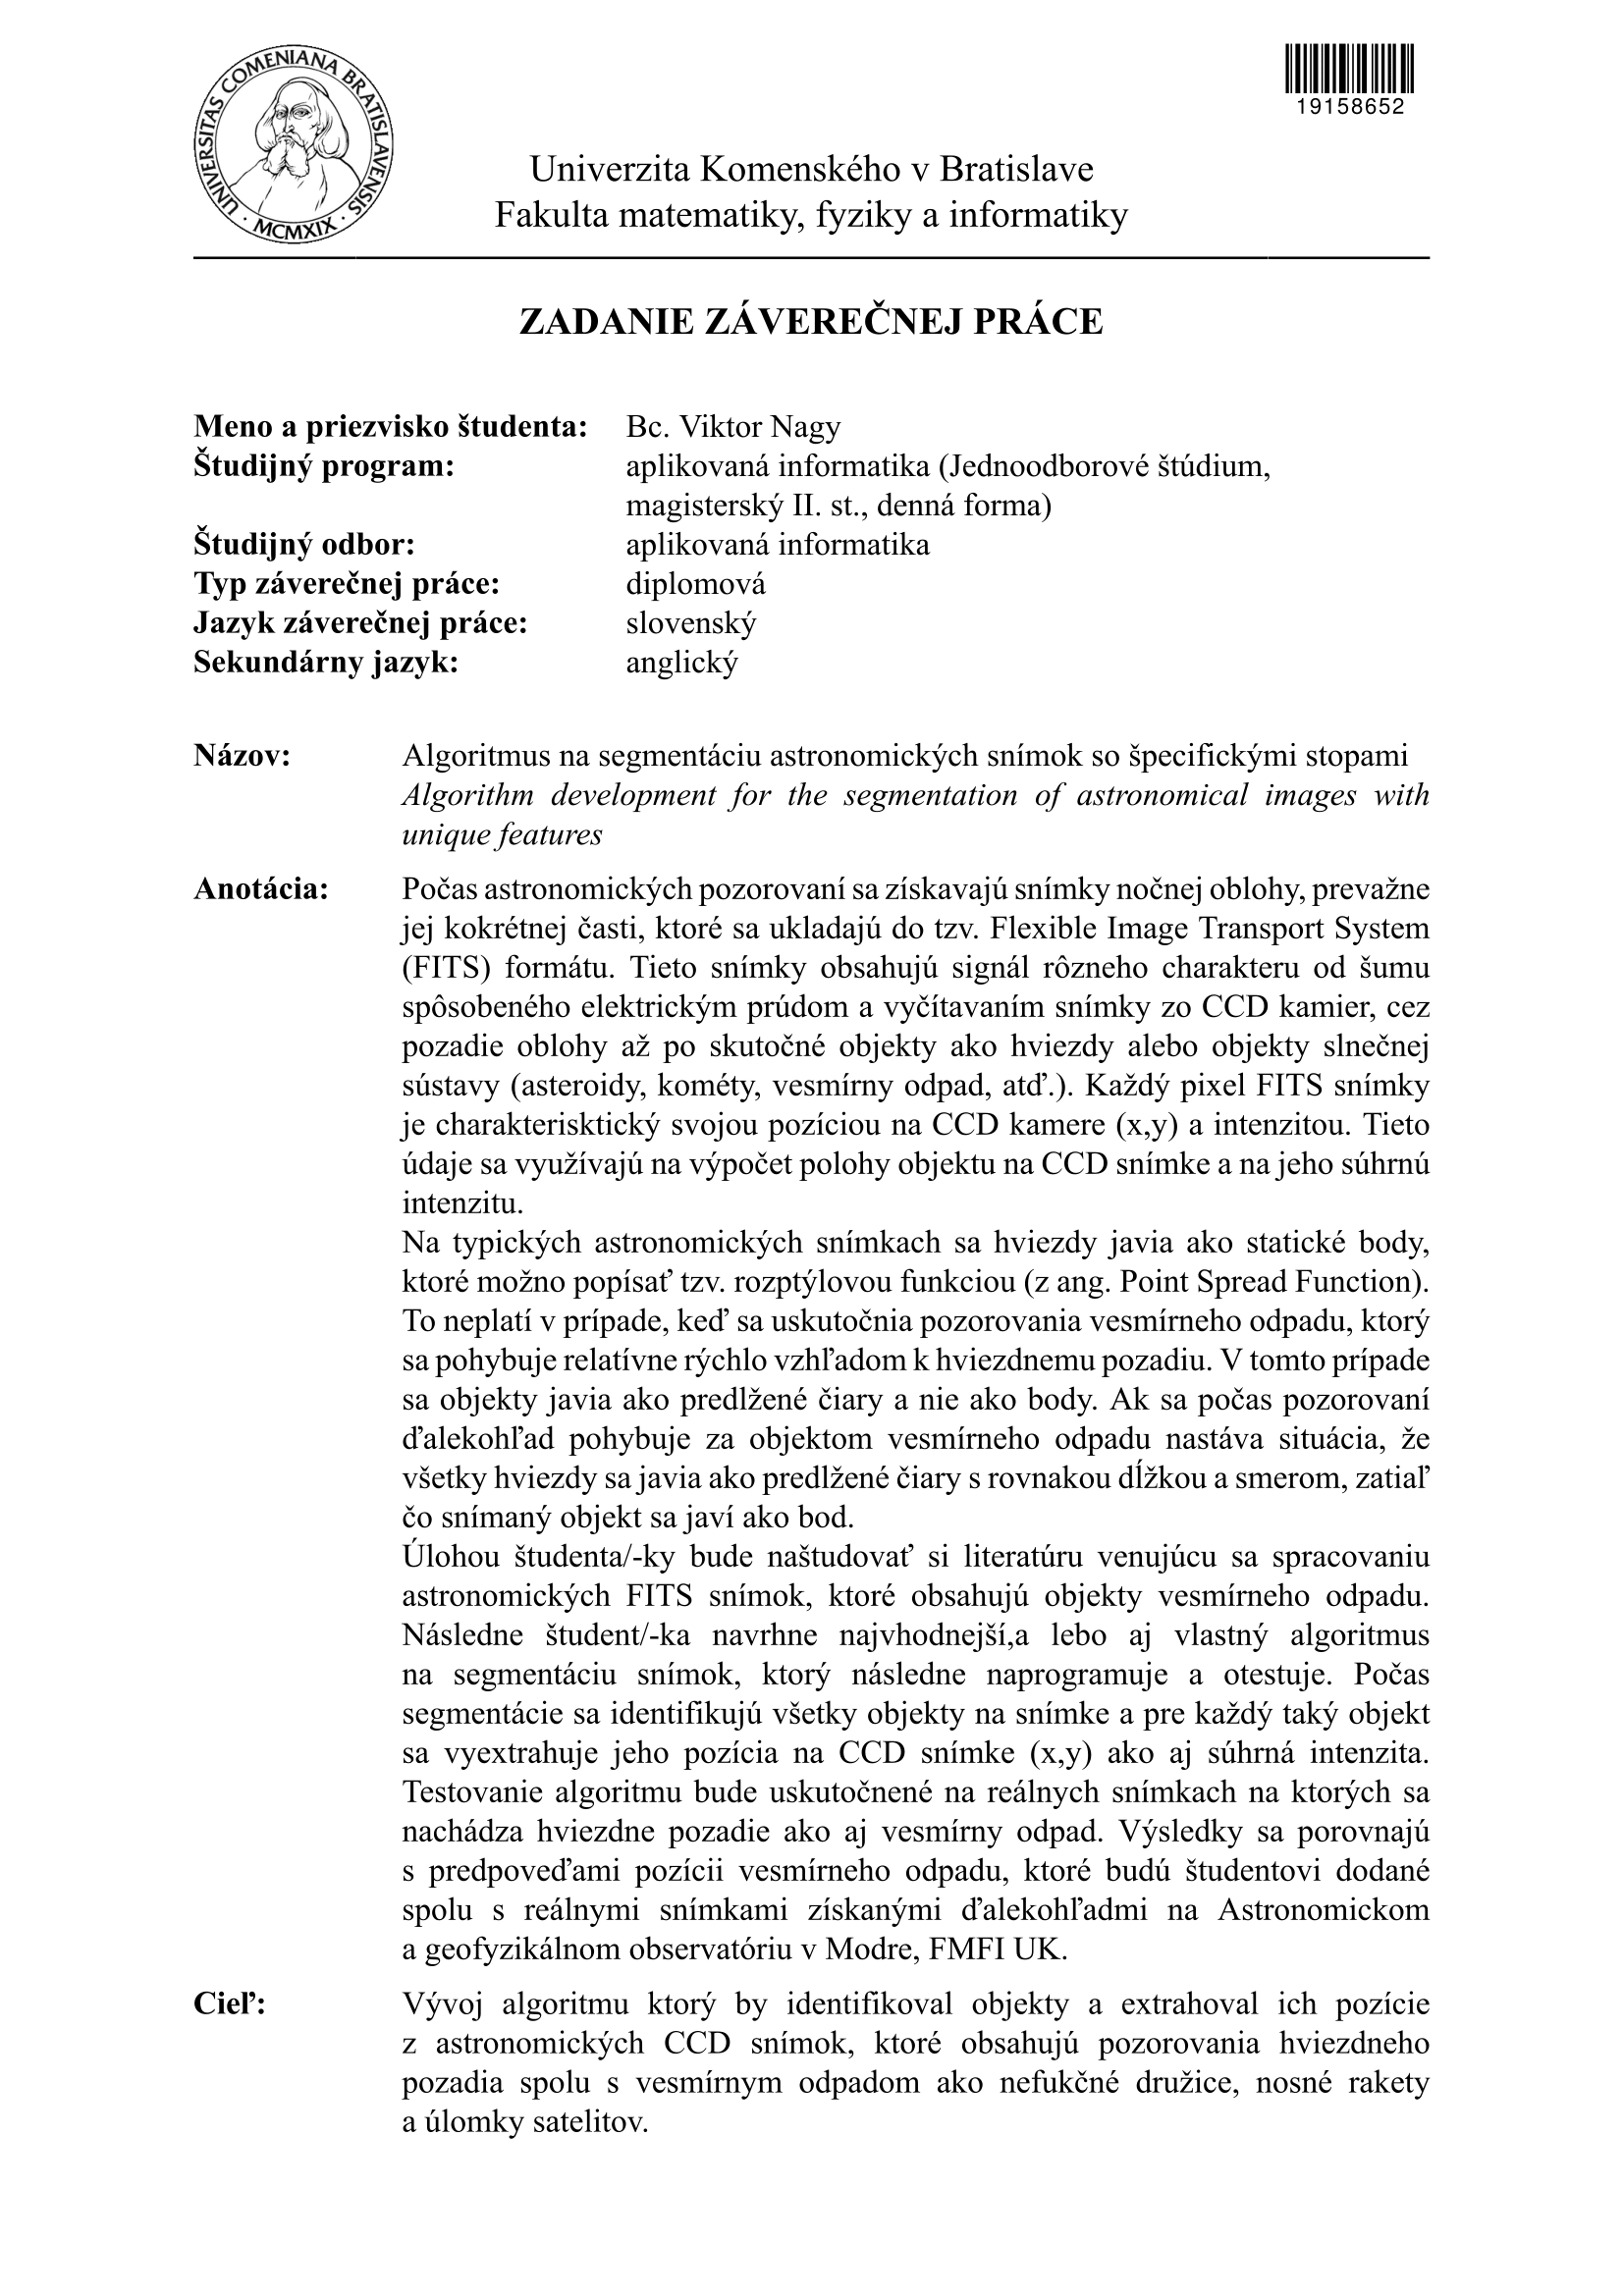
\includegraphics[width=\paperwidth]{zadanie1.png}}
\label{img:zadanie}
\end{center}
\end{figure}

\begin{figure}[H]
\begin{center}
\makebox[\textwidth]{
\includegraphics[width=\paperwidth]{zadanie2.png}}
\label{img:zadanie}
\end{center}
\end{figure}


\noindent
\begin{minipage}{0.25\textwidth}~\end{minipage}
\begin{minipage}{0.75\textwidth}
I hereby certify that this thesis has been composed by me and is based on my work.
All references and verbatim extracts have been quoted and all the data and images used have been specifically acknowledged.
No other work has been used in this thesis without giving credit to the original author.
\newline \newline
\end{minipage}
\vfill
~ \hfill {\hbox to 6cm{\dotfill}} \\
\mfplacedate \hfill \mfauthor
\vfill\eject
% koniec prehlasenia

\pagestyle{empty}
\chapter*{Acknowledgement}\label{chap:thank_you}
I would like to thank my supervisor Mgr. Jiří Šilha, PhD. for his input and guidance.
His invaluable expertise in astronomy and astrophysics was essential to successfully finish this thesis.
I would also like to thank my consultant prof. RNDr. Roman Ďurikovič, PhD. for his insights in image processing part of this thesis and for his organisation of YACGS seminary where we discussed progress as well as ideas that proved to be valuable during implementation of the thesis.
\vfill\eject
% koniec podakovania


\chapter*{Abstract}\label{chap:abstract_en}
During the astronomical observations images are acquired in so-called Flexible Image Transport System (FITS) format.
These images need to be processed and all the data about objects found in the image need to be exported for purpose of identifying them and determining their location.
Objects found can have point-like shape in case of stars or asteroids and can be described by the Point-Spread Function (PSF).
This does not apply to observations of space debris where objects take shape of streaks (trail-like objects) as they move comparably faster relative to the background.
This is only the case of sidereal tracking where telescope compensates the movement of the Earth while in object tracking situation reverses.
This document contains summary of prerequisite knowledge in given problematic, such as theory behind space debris as well as existing solutions.
While these images can contain background noise that distorts the data, we firstly focus on flattening of the image.
Then, we focus on segmentation and object detection discussing existing alternatives and implementing PSF based solution.
This solution is then tested on real data from the Astronomical and Geophysical Observatory in Modra (AGO) and validated by comparing our results to well established astronomical tool and the ground truth.
In the last part we discuss implementation including objects and methods needed to produce output in required ASCII form.


~\\
Keywords: debris detection, image processing
\vfill\eject

\chapter*{Abstrakt}\label{chap:abstract_sk}
Počas astronomických pozorovaní sa získavajú snímky v tzv. Flexible Image Transport System formáte.
Tieto snímky musia byť spracované a všetky dáta o objektoch nájdených na snímke musia byť exportované aby bolo možné dané objekty identifikovať a zistiť ich pozíciu.
Nájdené objekty môžu mať tvar bodu v prípade hviezd alebo asteroidov a môžu byť definované tzv. rozptylovou funkciou (z ang. Point-Spread Function).
Nie je tomu tak v prípade pozorovaní kozmického odpadu, ktorý má tvar čiary pretože sa hýba porovnateľne rýchlejšie k pozadiu.
Platí to len v prípade, že teleskop kompenzuje pohyb zeme tak aby hviezdy ostali na tom istom mieste počas celej doby uzávierky.
V opačnom prípade sa situácia mení a hviezdy naberaju tvar čiary zatiaľ čo kozmický odpad tvar bodu.
Tento dokument obsahuje zhrnutie teórie o danej problematike ako napríklad teória o kozmickom odpade ako aj existujúce riešenia.
Keďže snímky obsahujú nerovnosti v šume pozadia, najprv sa sústredíme na vyrovnanie tohto šumu aby sme zabránili skresleniu výsledkov.
Neskôr sa sústredíme na segmentáciu snímky a detekciu objektov kde opíšeme alternatívne riešenia a impelementujeme riešenie založené na rozptylovej funkcii.
Toto riešenie potom testujeme na skutočných dátach z Astronomického a Geofyzikálneho observatória v Modre (AGO) a validujeme výsledky porovnávaním s všeobecne uznávanými nástrojmi ako aj skutočnými výsledkami (v prípade syntetických snímkov).
V poslednej časti preberieme implementáciu, všetky metódy, triedy a ich premenné potrebné na vyprodukovanie výsledku v ASCII forme.
~\\
Kľúčové slová: kozmický odpad, spracovanie obrazu
\vfill\eject

% koniec abstraktov

\tableofcontents
\mainmatter

\pagestyle{headings}

\chapter{Motivation}

More than 60 years ago, humanity acquired ability to create artificial satellites and ever since, number of launches and consequent deployment activities are increasing.
Even thought scientists had multiple decades to fine tune this tremendous task, we are still far from reaching perfection.
Our inability to get cargo on the orbit without leaving a trail of parts behind lead to formation of space debris scattered around the Earth \cite{klinkrad}. \\
While solutions to this problem were announced already, it is essential to detect and consequently locate debris to make any effort in cleaning of our orbit possible.\\
In the meantime, avoiding collisions between satellites and debris is our top priority, demanding correct detection as well.
Detection of space debris poses multiple problems to solve starting with capturing of an image and ending with exact positions of objects in the orbit.\\
In this thesis we focus on two parts of this task - estimating and subsequent flattening of the background noise and then mathematically describing objects detected.

\chapter{Introduction}

\section{Space debris, definition}

Space debris are all man made objects, including fragments and elements in orbit or re-entering the atmosphere, that are non functional.
After more than 60 years of space program and more than 5250 launches, space debris comes in different shapes and composition \cite{esa_debris_numbers}.\\
This material is therefore hard to categorize differently than by it's means of creation \cite{klinkrad}. \\
\begin{itemize}
    \item Mission related objects and rocket bodies
    \item Fragments
    \item Non-functional spacecraft
    \item Other sources
\end{itemize}
    First category consists of objects that launches leave behind.
These objects are considered to be the largest of all the categories \cite{fmpi_cu}.
In extreme conditions during launch it is close to impossible to collect everything that is no longer needed for continuing of the mission.
Every cargo deployment or detachment leaves some sort of debris behind that would be inefficient to collect, because it would increase fuel needed as well as overall complexity of the hardware and software needed.
This category consists of material used to cover cargo hold, adapters holding rocket stages together as well as spent stages themselves.
This part of space debris is ought to change in the future, since it is easily considered littering, but steps were made already in form of reusable rockets.\\
    Fragment debris is the unintentional opposite of mission related objects.
This type of debris is created when spacecraft is scattered during impact with another orbiting object or by accidental explosion \cite{agapov}.
Spacecrafts usually contain some residual fuel that remains in tanks and over time, harsh environment of earth orbit can cause them to lose their mechanical integrity.
As a result, thousands of small parts are ejected with increased velocity away from the explosion.
As of 2018 there are approximately 750 000 fragments of size more than 1cm.
Fragmentation is not always accidental. In the January 2007 the Chinese FengYun-1C used surface launched missile to destroy satellite increasing the total number of space debris by 25\% \cite{lambert}.\\
    Non-functional spacecraft consists of all the objects that had some use in the past but are no longer operational.
Approximately 24\% of all cataloged objects are satellites, but more than third of those have no longer any use (ESA 2018).
These objects are expensive to remove since it would need a separate launch to remove them resulting in more possible debris.
According to Mitigation Guidelines released in 2002 by Inter-Agency Space Debris Coordination Committee (IADC) spacecrafts should be build with extra fuel to change their orbit after they are no longer operational.
Spacecrafts in Low Earth Orbit (LEO) should be slowed down until their altitude decrease lets them burn in atmosphere and spacecrafts in geostationary orbit (GEO) should be moved to higher orbit to avoid any unnecessary collisions with operational satellites.\\
In January 1, 2002 it was estimated that 31.8\% of all the debris is payload, 17.6\% spent rocket upper stages and boost motors, 10.5\% were mission-related objects, and the remainder of 39.9\% were debris with fragmentation origin where 28.4\% consists of upper stage collision and 11,5\% from colliding satellites (Klinkrad, 2002).

\section{The trend}


According to the trend seen in Figure 2.1, we can clearly conclude that number of debris is rising.
Graph shows that overall count is rising in exponential fashion that is reaching it's knee of exponential growth - the part where the exponential trend becomes noticeable.
We can therefore conclude that while number of annual launches increases, debris count will follow the same trend.
This makes detecting of already present debris vital for slowing down the trend to avoid creating more fragmentation debris.
Our long term goal is to avoid Kessler syndrome as proposed in 1978 by NASA scientist Donald J. Kessler \cite{kessler}.
He described the consequences of a self-sustained growth of the space debris, initially triggered by collisions between intact objects and ultimately sustained by collisions between fragments.
If this scenario would become reality, it would create impenetrable barrier that would render creation of new satellites as well as exploring the solar system inconceivable.

\begin{figure}[!hbt]
    \begin{center}
        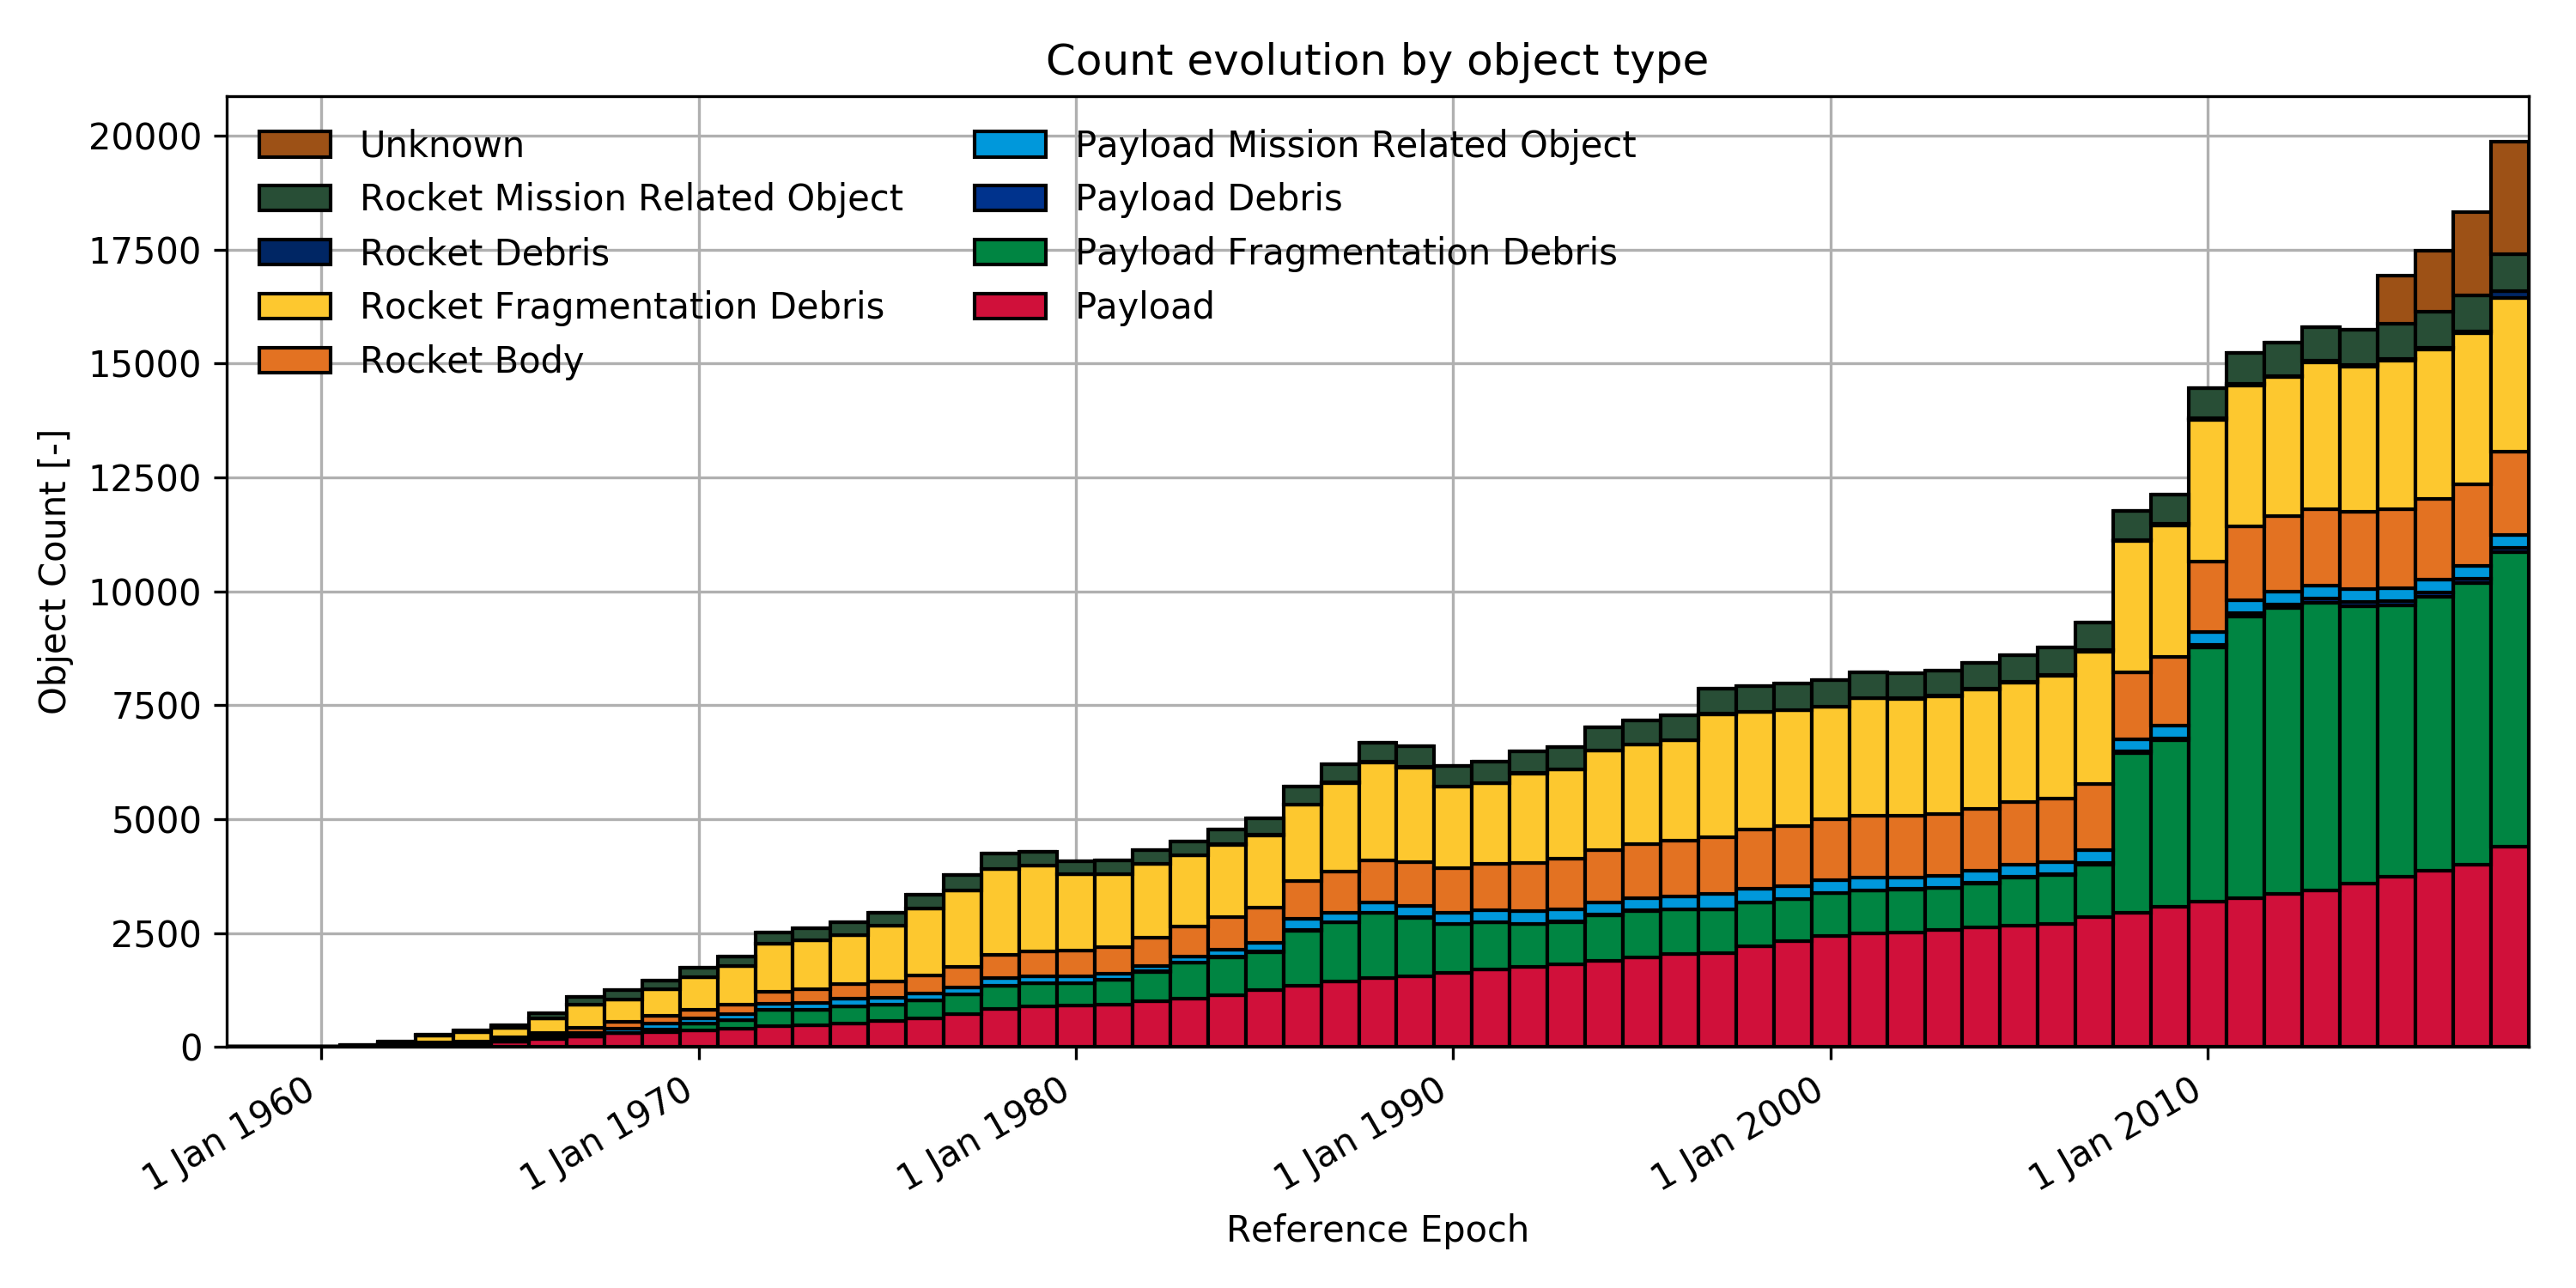
\includegraphics[scale=0.60]{images/debris_count.png}
        \label{img:debris_count}
        \caption{Evolution of debris count over time \cite{esa_about_space_debris}}
    \end{center}
\end{figure}


\section{Spatial distribution}

\say{Within the domain of the solar system all planets describe elliptical paths with the Sun at one focus \cite{kepler}}
\begin{flushright}
    Johannes Kepler, 1st Kepler's law
\end{flushright}
The same law applies to geocentric motion as well, meaning that any object describes elliptical path with the Earth at one focus.
\\

\subsection{Types of orbits}

Objects orbiting earth can be categorized by its position as follows:
\begin{itemize}
    \item{Low earth orbit (LEO)}
    \item{Geosynchronous equatorial orbit (GEO)}
    \item{Global navigation satellite system (GNSS), Highly-elliptical orbit (HEO), Geosynchronous transfer orbit (GTO), Molniya}
\end{itemize}

LEO is the most dense part of earth's orbit creating sphere-shaped layer of debris.
It consists of more than 10000 objects, mostly fragments.
Figure 2.2 shows position of the orbits(a) as well as aproximate location of objects(b).
\\
GEO, with mean altitude of 35 786km, forms ring-like shape over Earth's equator.
Cataloging objects in this orbit is more problematic and only object with size of 50cm are reflecting enough light to be detected from earth's surface.
In this thesis we will mostly focus on objects present in GEO.
\\

\begin{figure}[h]
    \centering
    \subfloat[Types of orbits]{{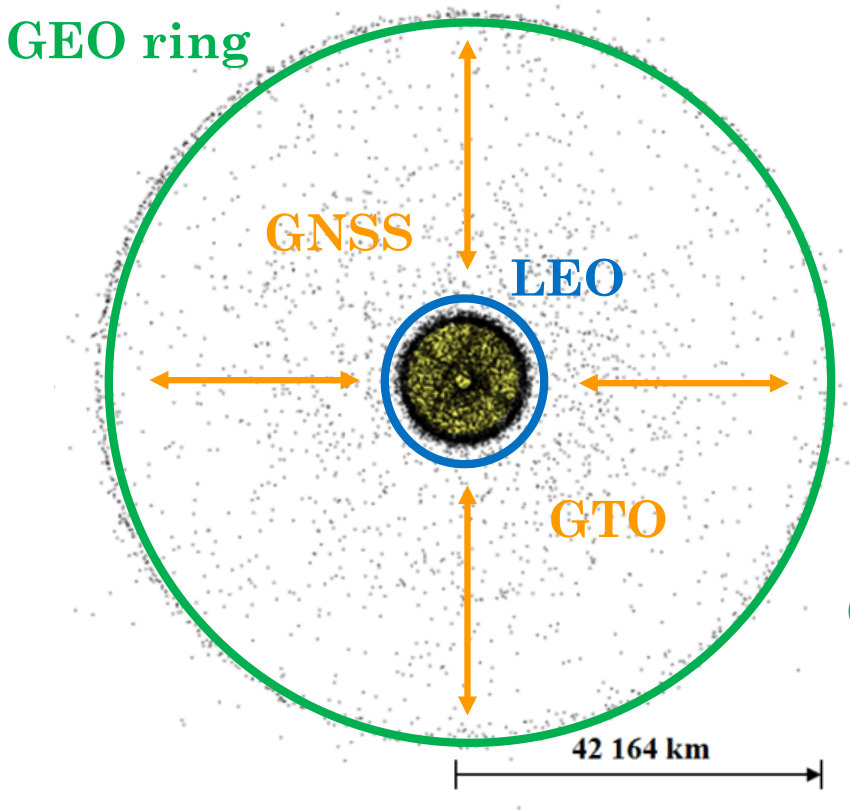
\includegraphics[width=5cm]{images/geo_leo.png} }}%
    \qquad
    \subfloat[Aproximate density]{{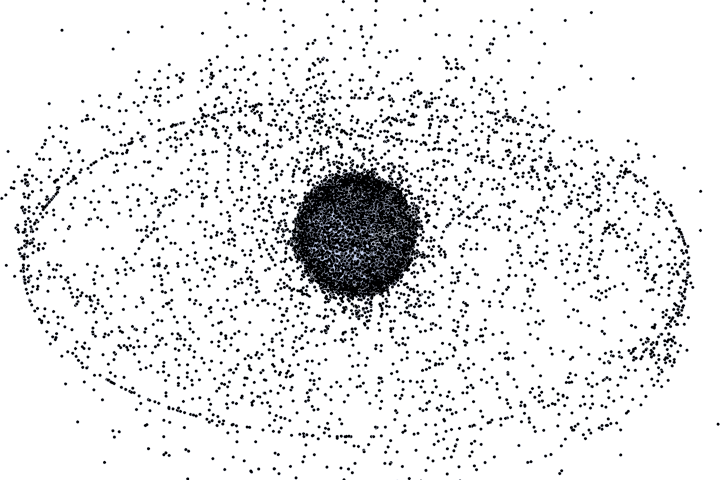
\includegraphics[width=5cm]{images/junk.png} }}%
    \caption{Space debris distribution (Courtesy of Jiří Šilha)}%
    \label{fig:example}%
\end{figure}

\section{Data collection}

\subsection{FMPI AGO}
All the data used in this thesis is captured in Astronomical and Geophysical observatory in modra (AGO) from the main telescope with these basic features:
\begin{itemize}
    \item{Newtonian reflector with parabolic mirror}
    \item{0.7m primary mirror}
    \item{2.9m focal length}
    \item{28.5x28.5 arc-min field of view}
    \item{equatorial mount}
    \item{resolution 1024x1024 pixels}
\end{itemize}

\begin{figure}[!h]
    \begin{center}
        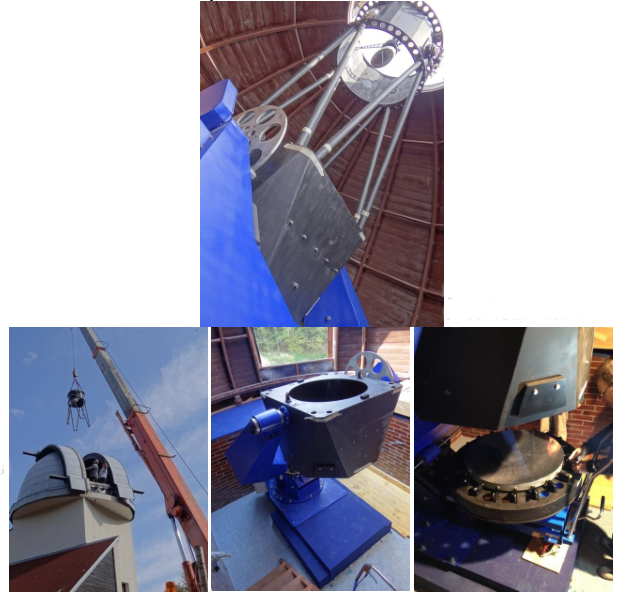
\includegraphics[scale=0.35]{images/telescope.png}
        \label{img:telescope}
        \caption{70cm telescope in AGO modra (FMPI CU)}
    \end{center}
\end{figure}

\subsection{Fits format}
Images coming from AGO are in form of FITS files (Flexible Image Transform System) \cite{fits}.
It is standardized format for astronomical observations consisting of header and data.
Header is data structure similar to dictionary or map from string to string.
It consists of multiple key/value pairs containing useful information about the image.
Data part of the FITS file contains array of arbitrary size containing intensity values of given pixels.
In our case data has size of 1024x1024 pixels.
It is important to state that in this data array we are using two axis to determine position of the pixel.
In reality, object present on any particular position in this data array is real object which position can be specified with spherical coordinate system as described in Section 2.4.4.
For purpose of this thesis we are using this data and one header values to give algorithm additional information about the image that is used in object detection.

\subsection{Tracking types}
We differentiate 2 types of tracking
\begin{itemize}
    \item{Sidereal tracking}
    \item{Object tracking}
\end{itemize}

Telescope uses 5 seconds exposure and during this time it can either compensate for Earth's motion to remain in sync with stars in the background (sidereal) or it can move freely with earths rotation.
During sidereal tracking, stars remain point-like while any object moving on Earth's orbit traces streak-like path.
In object tracking, polar opposite is the case resulting in points in place of orbital objects, and streaks in case of stars in the background.

\begin{figure}[H]
    \begin{center}
        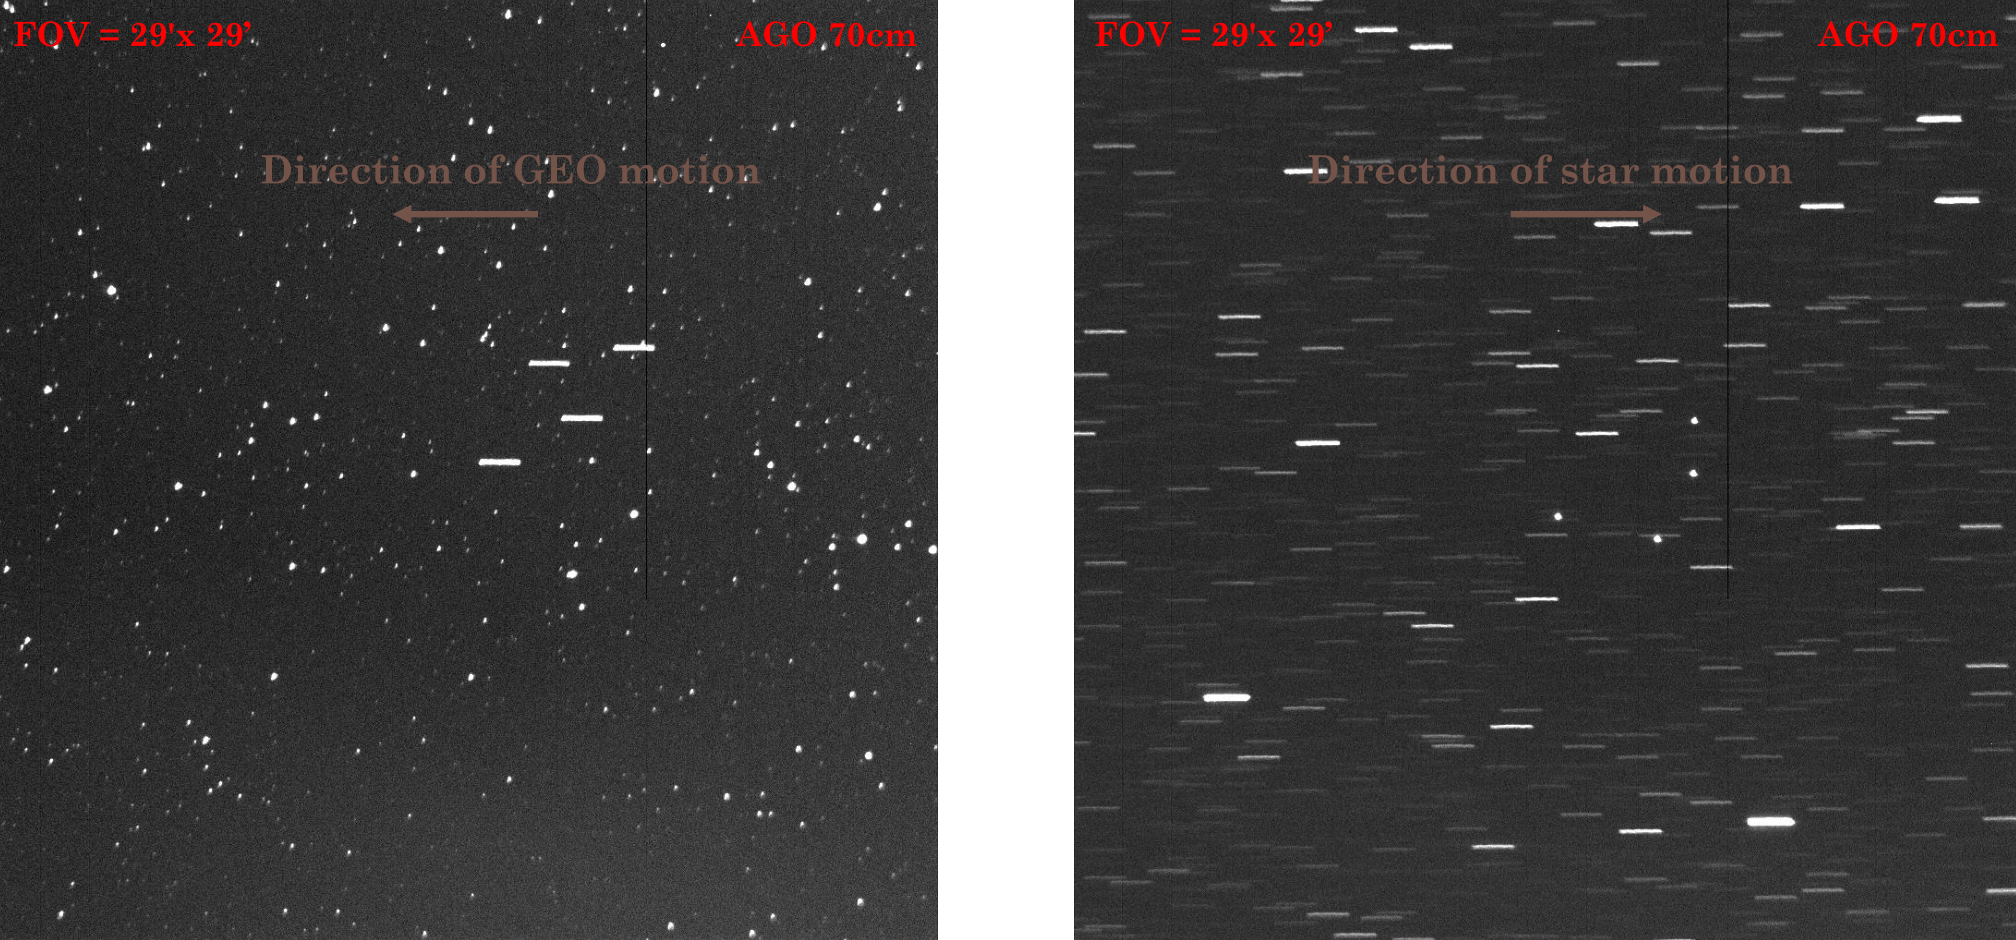
\includegraphics[scale=0.60]{images/tracking.png}
        \label{img:tracking types}
        \caption{Difference types of images with sidereal tracking (left) and object tracking (right). Courtesy of Jiří Šilha.}
    \end{center}
\end{figure}

Data part of the fits file consists of array with size 1024x1024 pixels containing total intensity captured during exposure.

\subsection{Equatorial coordinate system (RADEC)}
This coordinate system is commonly used in astronomy, often referred to as spherical coordinate system.
It's acronym comes from the 2 coordinates that this system uses
\begin{itemize}
    \item{Right Ascension}
    \item{Declination}
\end{itemize}
Declination specifies the angular distance of object perpendicular to equator.\\
Right ascension specifies the angular distance of the object eastward from the vernal equinox with angular distance measured in hours.
In this context one hour is equal to 15 degrees.\\
For the purpose of this thesis we are considering objects in the image as points on the X and Y axis, but while our aperture operates in RADEC coordinates and final position of objects after entire pipeline is also in this coordinate system, it is important to understand the difference between the two.
\section{Pipeline definition}

The whole processing pipeline starts with capturing of the image and ends with record of space debris and it's RADEC coordinates.
Pipeline consists of following steps \cite{silhaetal}
\begin{itemize}
    \item{Image reduction}
    \item{Sky background estimation/extraction}
    \item{Objects search and centroiding}
    \item{Star field identification}
    \item{Astrometric reduction}
    \item{Star Masking}
    \item{Tracklet building}
    \item{Object identification}
    \item{Data format transformation}
    \item{Output data redistribution}
\end{itemize}
\par
\indent
Captured image in it's raw form is not usable for later stages of pipeline, therefore it needs to be cleaned of as much noise as possible.
During image reduction, we take the image with closed lid of the telescope to capture any noise created by aperture itself.
This process removes noise created by difference in sensitivity of pixels, dust present on the optical system as well as noise created by current.\\
\indent
Process of image reduction is not perfect and some noise remains, but most of the noise after this step comes from external sources.\\
\indent
Sky background estimation tries to create map of background noise.\\
After this map is created, it gets subtracted from original image, removing all global and local gradients.\\
This process can never remove all of the noise, but flattening of the noise is vital for latter steps.\\
\indent
Star object identification locates x,y positions of stars in the image.\\
These stars are then covered because they are not objects of our interest.
While some stars are too weak to be labeled correctly, later processing needs to follow.\\
\indent
After stars are removed, we start segmenting objects of interest.\\
We then add another dimension to the problem, considering correlations of objects across images taken in different time - tracklet building.\\
\indent
The final product consists of tracklet with RADEC coordinates, therefore final conversion from x,y coordinates is needed.\\
\\
The goal of this thesis is to focus on 'Sky background estimation/extraction' and 'Objects search and centroiding'.
These steps are essential in obtaining correct results in both objects position as well as it's apparent magnitude.
Every step of the pipeline after these two depend on the correct results, therefore those are the main focus of the thesis.
On the other hand, 'Image reduction' - step before background estimation - is well defined problem with known solutions.

\chapter{Sky background estimation and extraction}
A lot of a noise present in captured images is unavoidable consequence of CCD(Charge-coupled device) that is used during capture. Although this noise can be removed during early stages of preprocessing with bias images, some noise remains because it comes from external sources.\\
There are several sources of external noise
\begin{itemize}
    \item{Moon light (global linear gradient)}
    \item{Stars, Nebulas, Galaxies (local nonlinear gradients)}
    \item{Remnants of hardware related reflections, stray light}
\end{itemize}
Two basic algorithms are used to extract background from the image.

\section{Median filtering}

This method is very simplistic and suffers few disadvantages \cite{stovaken}.
Idea behind this method is to use 2-d convolution with median kernel of size at least 0.2 times the original image \cite{median_filtering}.
As a result of this convolution process, blurred version of the original image is being created.
Main advantage of this method is that it preserves faint objects and this effect increases with use of larger kernel sizes.
Obvious disadvantage of this method is that if we want to achieve usable results, large kernel needs to be used and this increases time of computation exponentially.
Version of this algorithm was implemented during this thesis but to archive any usable results, 20 to 30 seconds were spent in convolution computation.
It is important to specify that these time-spans were experienced on regular PC with single quad-core processor.
Algorithm will be implemented and used on Charon server in Modra with 16 cores and time spent would improve significantly but still we should always try to minimize time of execution when keeping in mind length of the entire pipeline.
Another disadvantage of this method is that it doesn't detect small local gradients and this effect only increases with kernel size.
The last but not least problem with this approach comes from very nature of convolution and with it's behavior near edges of the image.
Image after this process loses data on border of the image with width of half of the kernel size.

\section{Sigma clipping}

Sigma clipping takes different approach.
It consists of preprocessing and iterative clipping process \cite{kouprianov}.
We first need to define some parameters and other values used in this method.
\begin{itemize}
    \item{$\sigma$ - standard deviation}
    \item{$\overline{\Delta B_i}$ - mean deviation}
    \item{I(x,y) - intensity of the pixel x,y of the original image}
    \item{$B_0$(x,y) - intensity of the pixel x,y of initial the background estimate}
    \item{$B_i$(x,y) - intensity of the pixel x,y of i-th iteration of the background map}
    \item{B(x,y) - intensity of the pixel x,y of the resulting background map}
\end{itemize}

\subsection{Image preprocessing}
Sigma clipping method iteratively converges to the background map, but firstly it needs initial estimation to iterate over.
The initial estimation is created by downsizing of the image to 10\% of the original size using bicubic interpolation.
This helps with minimizing of aliasing artefacts.
After that we blur the downsized image with median filter, but in contrast to median filtering method, we use much smaller kernel size.
Next we upsize the image and smooth it out with convolution using gaussian filter.
The resulting image is then used in the next step of the algorithm.

\begin{figure}[!hbt]
    \begin{center}
        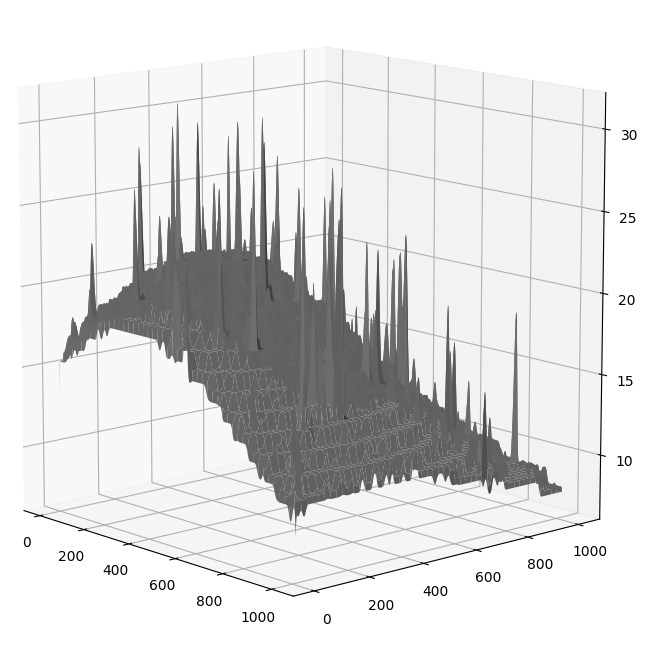
\includegraphics[scale=1.30]{images/background_initial_guess.png}
        \label{img:background_initial_guess}
        \caption{Map produced by initial estimation}
    \end{center}
\end{figure}

\subsection{Iterative process}
Preprocessed image already shows the global background trend, but it is far from being usable in this form.\\
We iterate the image with following equation \\
\begin{gather}
    \Delta B_{i+1} =
    \begin{cases}
        \Delta B_i(x,y) & |\Delta B_i(x,y)-\overline{\Delta B_i}| < 3\sigma_i\\
        \overline{\Delta B_i}& |\Delta B_i(x,y)-\overline{\Delta B_i}| >= 3\sigma_i\\
    \end{cases}
\end{gather}

The equation has 2 cases to consider depending on the difference between value of previous iteration (or estimated value in first iteration) and mean deviation compared to standard deviation.\\
The final product of background map is then computed with $n$ iteration as

\begin{equation}
    B(x,y) = B_0(x,y) + \Delta B_n(x,y)
\end{equation}

\begin{figure}[H]
    \begin{center}
        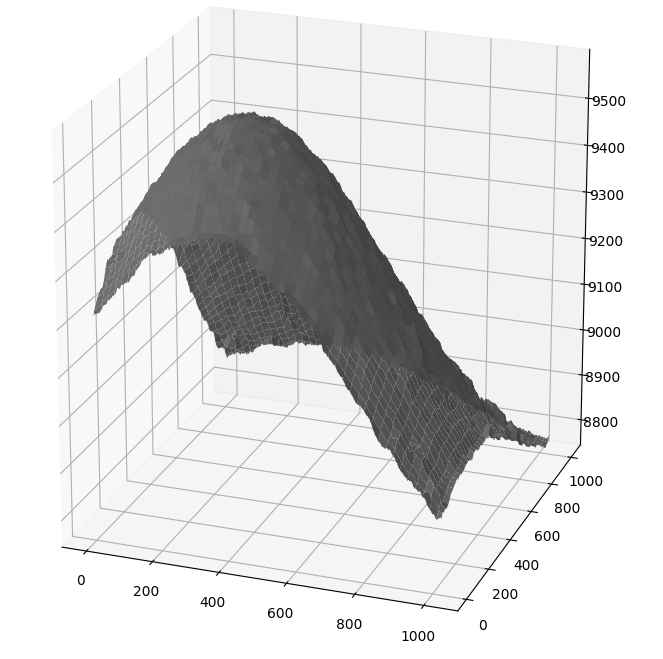
\includegraphics[scale=1.50]{images/3_iter_sigma.png}
        \label{img:background_initial_guess}
        \caption{Final result with 3 iterations}
    \end{center}
\end{figure}

Compared to median filtering this algorithm produces the background image faster and it's speed can be modified with proper choice of number of iterations.

\subsection{Parameter choice}
During implementation we experimented with all the parameters of the algorithm to obtain the best results possible.
We experimented with different sigma values used in case Equation 3.1 as well as changing of mean derivation to median.
Changes showed some promising results on test cases, but parameters being described above showed to be the most robust.\\
We also experimented with choice of preprocessing steps.
Best results were obtained with choice of kernel with size of 15x15.
This parameter choice showed best trade-off between speed of computation and minimizing artefacts on the resulting map.\\
Lastly we blurred the resulting image with box blur to completely remove any artefacts that could be produced during iteration.\\
Parameters and steps described in this section produced the most robust results across multiple test cases.

\clearpage
\begin{figure}
    \centering
    \subfloat[3 iterations]{{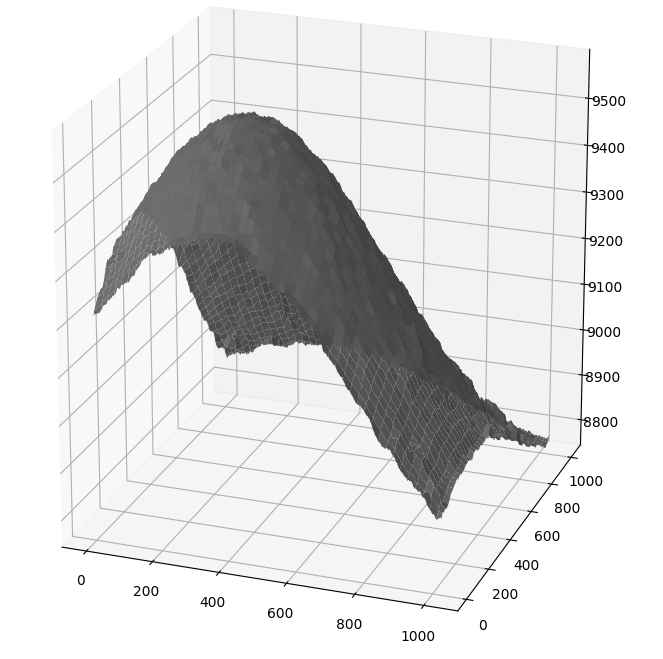
\includegraphics[width=5cm]{images/3_iter_sigma.png} }}%
    \qquad
    \subfloat[5 iterations]{{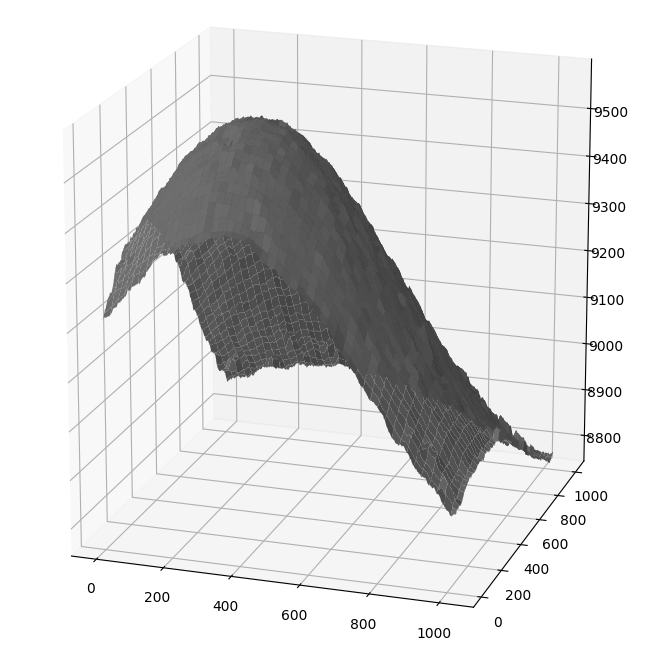
\includegraphics[width=5cm]{images/5_iter_sigma.png} }}%
    \qquad
    \subfloat[7 iterations]{{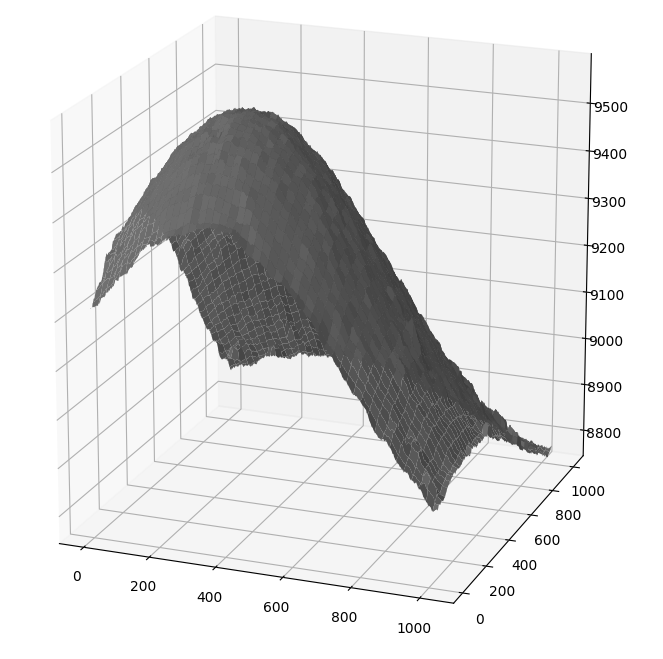
\includegraphics[width=5cm]{images/7_iter_sigma.png} }}%
    \qquad
    \subfloat[13 iterations]{{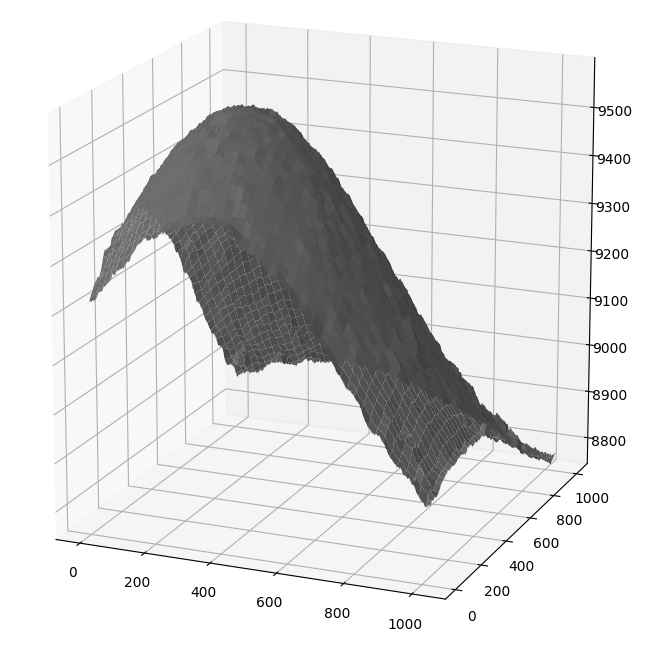
\includegraphics[width=5cm]{images/13_iter_sigma.png} }}%
    \caption{Comparison of different choice of number of iterations}%
    \label{fig:iterations}%
\end{figure}

Every image is unique, therefore in the final implementation, number of iterations is parameter to choose, but 3 iterations seem to be reasonable default value.


\begin{table}[H]
    \centering
\begin{tabular}{|l|l|}
\hline
                  & sigma               \\ \hline
after iteration 1 & 327.226637 \\ \hline
after iteration 2 & 248.904670 \\ \hline
after iteration 3 & 248.255926 \\ \hline
after iteration 4 & 248.255926 \\ \hline
\end{tabular}
    \caption{Change of sigma after iterations}
    \label{tab:sigma}
\end{table}

We can observe from Figure 3.3 and Table 3.1 that increasing number of iterations after some threshold doesn't affect results.\\
The biggest change occurs in the first iteration and every subsequent iteration after third changes sigma negligibly.\\

\begin{figure}[H]
    \begin{center}
        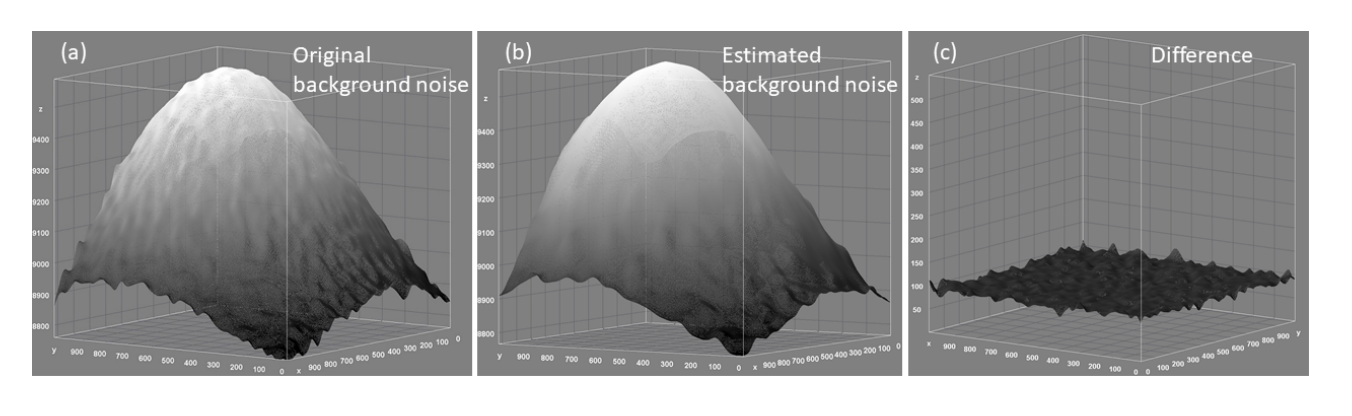
\includegraphics[scale=1.20]{images/sigmaclip_difference.png}
        \label{img:background_result}
        \caption{Synthetic background, background extracted from image, difference \cite{silhaetal}}
    \end{center}
\end{figure}

For easier comparison we created multiple synthetic noises to simulate background with known solution.
On the Figure 3.4 we have synthetic background (a), estimated background (b), and their difference (c).
We can observe that algorithm extracts shape of the background correctly and leaves only linear noise.

\section{Grid sigma clipping}
During implementation we considered use of sigma clipping in different manner.
The core idea was splitting the image into sections generating $n$ columns and $m$ rows.
This approach creates $n \times m$ sub-images each with size
\begin{equation}
    (width_{original}/n) \times (height_{original}/m)
\end{equation}
with and possible extra pixel in last row (or column depending on considered dimension) if size of the image is not even.
The main hope behind this approach was to make sigma clipping algorithm more robust to small background gradients with added option to choose these parameters.
This would give us option to detect even the smallest of the background phenomena.
Version of this algorithm was implemented during the implementation part of the this thesis.


\begin{table}[H]
    \centering
\begin{tabular}{|l|l|l|}
\hline
                  & cumulated difference & mean difference\\ \hline
    no grid & 97969264.02840663 & 93.47484103256222 \\ \hline
    10x10 & 98015474.91055997 & 93.43077090111412 \\ \hline
    30x30 & 97968103.14388879 & 93.42966379536513  \\ \hline
    50x50 & 97976495.76744124 & 93.43766762489437 \\ \hline
\end{tabular}
    \caption{Absolute and mean difference between background generated by algorithm (with multiple grid variations) and original synthetic background}
    \label{tab:grid_results}
\end{table}


As observed by absolute difference metric in Table 3.2, this approach shows bigger absolute difference then original non-grid version, but only at small grid numbers. Nevertheless grid version outperformed non-grid version on $30 \times 30$ run.
We can see some improvement but it comes with a cost.
Separation of the image into smaller segments takes extra time although performance hit is minimal.
Real negative side of this approach lays in the last part of the process, joining all the pieces of the background back together.
This creates step-like relics on lines where the image was cut.
These relics demand another smoothing at the end to fix this irregularity, distorting the data.
Clearly, some improvement can be achieved but improvement is minimal.

\begin{figure}[H]
    \begin{center}
        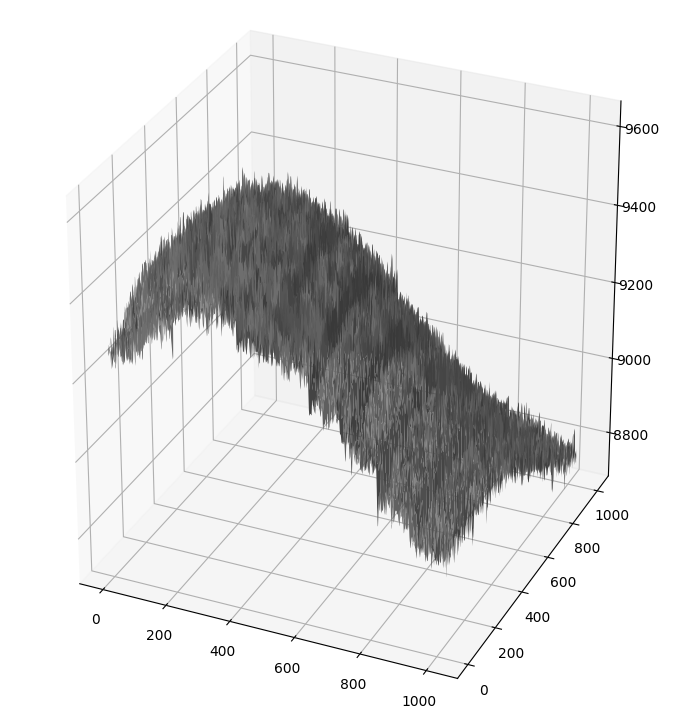
\includegraphics[scale=0.50]{images/grid_steps.png}
        \label{img:grid_steps}
        \caption{Grid steps, joining artefacts ($10 \times 1$ grid)}
    \end{center}
\end{figure}

In Figure 3.5 we can observe steps before smoothing, clearly showing additional data distortion.
Example used separates the image into $10 \times 1$ sections to make steps more visible because of their one dimensional nature.\\
\\
In the results we decided not using grid version of the algorithm because advantages are minimal while cost in performance as well as increasing chance of data distortion outweights the benefits.
Also separation into more subsections increases this risk exponentially.

\section{Sequential execution}
During testing phase of the algorithm we experimented with multiple runs of algorithm in sequence.
While extraction of background from the image is essential in some cases, it comes with a cost.
By using this algorithm we remove some of the intensity from the image.
We subtract the extracted background map from the original image and by doing so we shift all the values to lower ones.
This is desired behavior and does not distort data for further processing because relative difference between objects and noise remains unchanged.
The real data distortion of this method comes from the fact that our estimated background contains noise.
While objects high enough above noise level are unaffected by this subtraction, some objects with small intensity values might get subtracted away.
Sequential execution on the result from previous execution will increase this risk substantially.

\chapter{Object search and segmentation}
After the image is background is flattened, we can start the segmentation process.

\section{Signal to noise ratio}
Signal to noise ratio(SNR) is measure that describes level of data as compared to level of the background noise.
It is calculated as \cite{snr}
$$ SNR = \frac{S}{\sigma} $$

where

\begin{itemize}
    \item $S$ - sum of all intensities of the data
    \item $\sigma$ - sum of all background intensities
\end{itemize}

For purpose of our final output, where we frame objects into rectangular segments, we prefer SNR to be defined with peak value in the object yielding the following equation

$$ PSNR = \frac{S_p-B}{\sqrt{S_p-B+b}} $$

where

\begin{itemize}
    \item $S_p$ - peak value of the signal
    \item $B$ - median of previously calculated background
    \item $b$ - dispersion of the noise
\end{itemize}

Before segmentation, we need to consider what SNR are we dealing with.
SNR can vary enormously, starting with values slightly over one but can reach values of hundreds.
Having high SNR is therefore very important in proper segmentation with good results but lower values can lead to impossible task, because if SNR is close to 1, data is indistinguishable from noise.\\
The data we used was created synthetically with SNR of 50 but we tested on real images as well where SNR varied.

\section{Segmentation methods}

From image processing point of view, we know at least these 3 solutions to the given problem \cite{kouprianov}

\begin{itemize}
    \item Barycenter positions
    \item Edge detection
    \item Point spread function
\end{itemize}
Variety of classical centroiding methods exist and are used among which the most widely used is "Center Of Gravity" \cite{wang} \cite{flewelling}.
Barycenter positions is considered to be the easiest to compute from the given options but has some major disadvantages.
Solutions deals with center of mass of the objects and it is calculated from the intensity values.
This is the main problem of the method, that shows most noticeably in trails shifting this centers multiple pixels if atmospheric turbulences creates these local fluctuations.
\\
Edge detection algorithms can be used to segment the data, but they suffer from the same data distortion as well as barycenter positions.\\
Both of these approaches were considered, but not implemented during this thesis.
The reason is that the latter shows the most robust results even at lower SNR, but mainly we need to fit functions to the objects to extract additional data such as standard deviation of function mimicking it's shape.\\
All of these methods consist of two steps
\begin{itemize}
    \item Noise/Objects separation
    \item Object description
\end{itemize}
We firstly need to separate data from the noise.
To extract objects of interest we use some metric that gives boolean result and apply it to the image.
Then we we describe these objects mathematically using Point Spread Function.

\subsection{Thresholding}

After reading literature we found that most of the solutions use simple thresholding value to separate data from the noise.
This solution gives good enough results but has some edge cases of usability that could be improved on.
During implementation we found some cases where use of this approach might be challenging.
If the data has global background gradient (but the same effect could be seen on smaller scale as well), finding single correct thresholding value would be impossible.
This issue is removed in most of the cases with background extraction algorithm, but in some cases with low SNR where loss of information is unbearable, we would not be able to do it.
\\
The idea is to transform our 2d image into 1d histogram.
While most of the values on the image can be attributed to the noise, we can observe separation between data and noise on the histogram.
Then we fit gaussian to this histogram.
After the gaussian with corresponding shape is found, we decide where to put our thresholding value.
When there is at least some separation between values of noise and actual objects (when SNR has reasonable high value) then we found that $2 * \sigma$ to the right from the maximum extracts the most of the noise and can be used as thresholding value. (where $\sigma$ stands for standard deviation of the gaussian fitted to the histogram).
The less SNR our image has, the more actual data will be captured by the fit.
This cannot be avoided but implementation contains option to show this fit and let user set $\sigma$ appropriately.
If SNR is low enough and noise cannot be clearly distinguished from the data by this method we considered another approach using sobel operator.

\begin{figure}[H]
    \begin{center}
        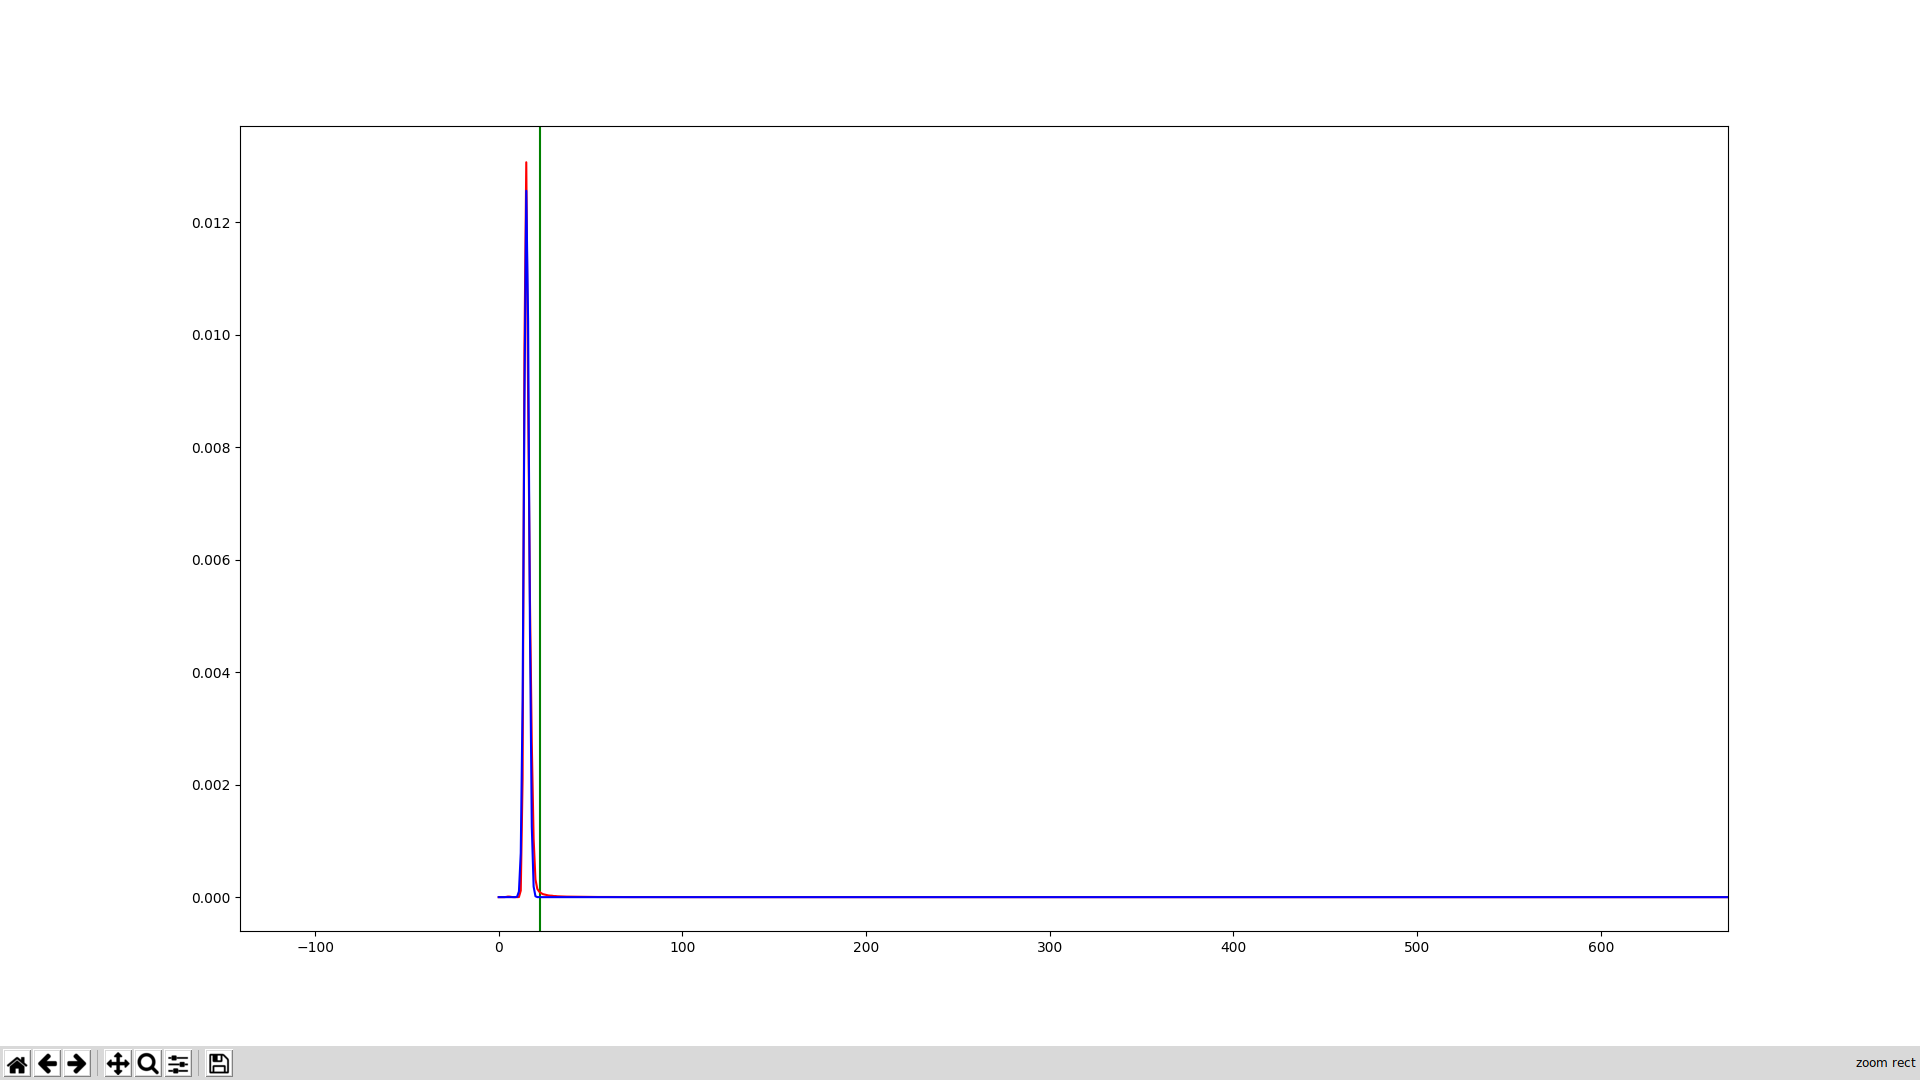
\includegraphics[scale=0.95]{images/hist_fit_far.png}
        \label{img:background_initial_guess}
        \caption{Example of fit to the histogram representation}
    \end{center}
\end{figure}

In the figure 4.1 we see that truly most of the values present in our image belong to noise region.
Blue color shows the trend of histogram, red color shows our estimated gaussian fit and green line shows the position of $2 * \sigma$ to the right from it's maximum value.

\begin{figure}[H]
    \begin{center}
        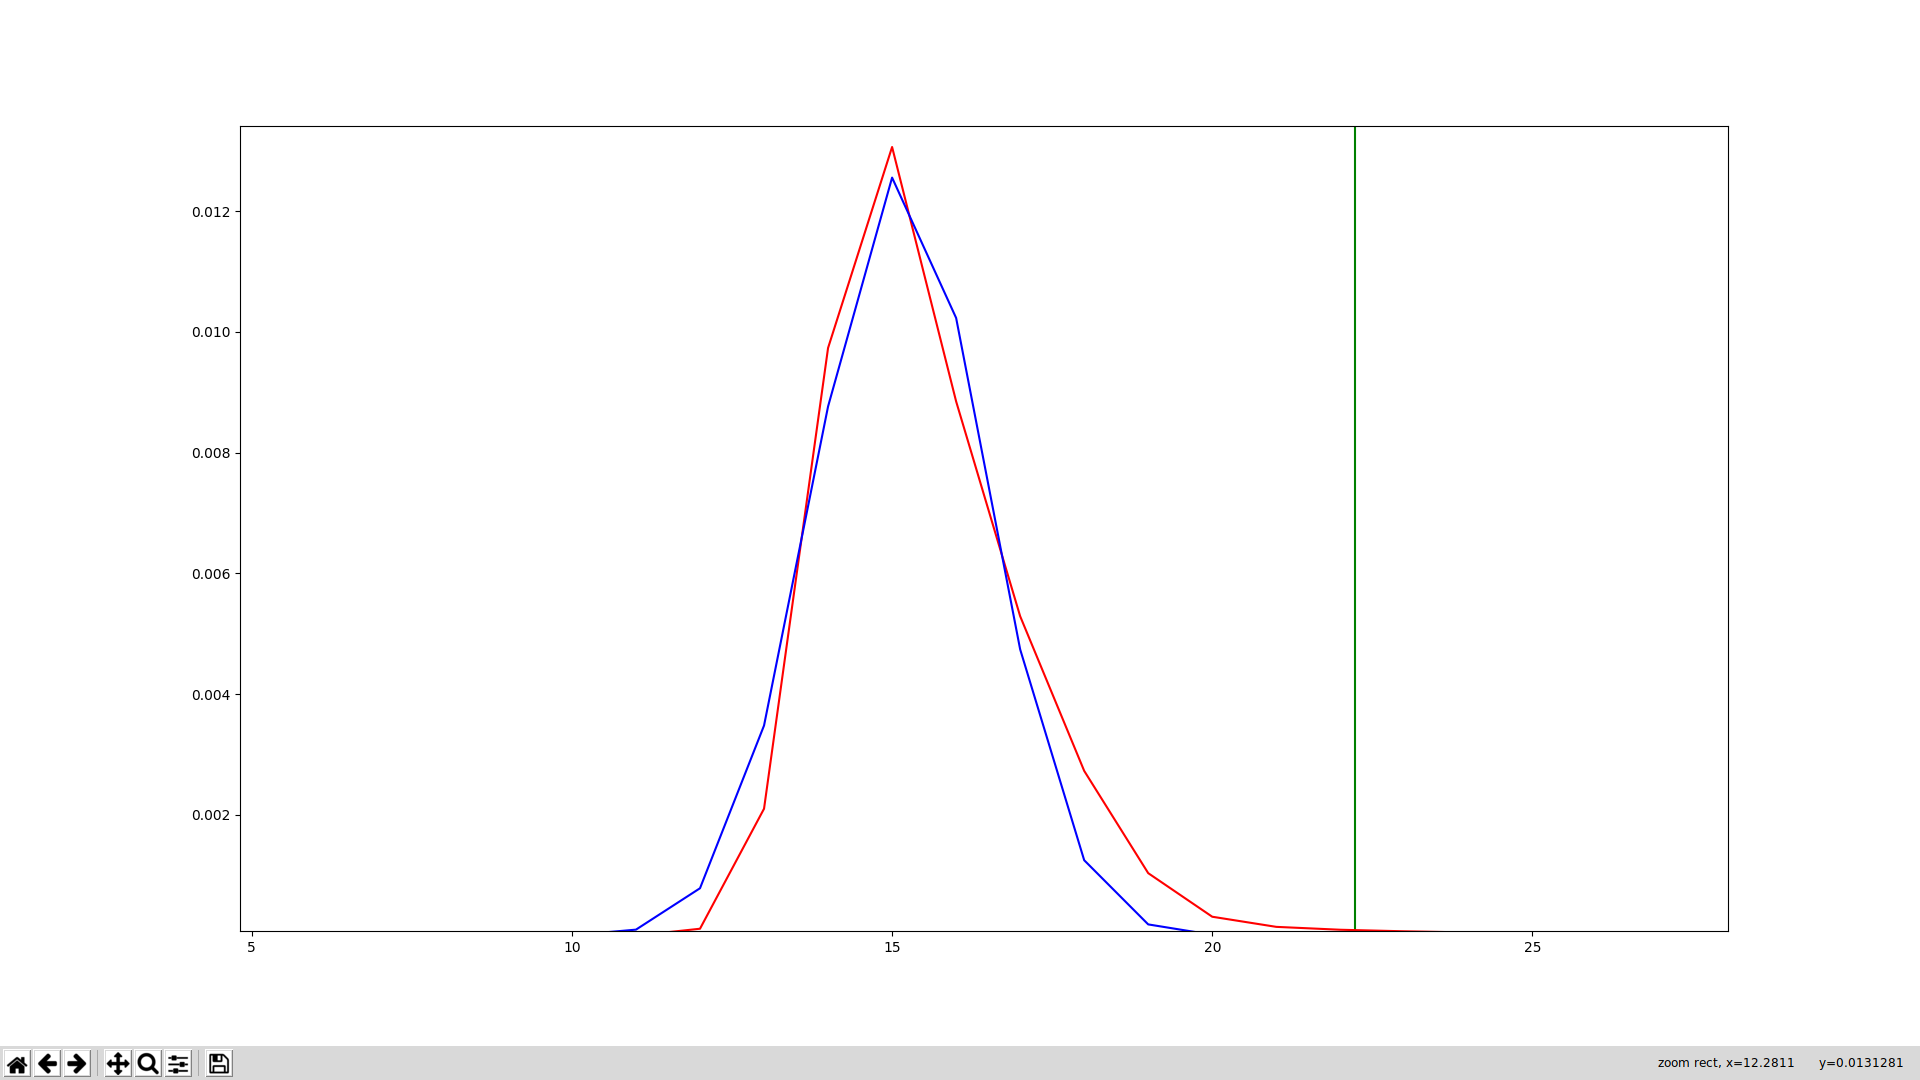
\includegraphics[scale=0.95]{images/hist_fit_close.png}
        \label{img:background_initial_guess}
        \caption{Closer look, showing position of noise around values 15}
    \end{center}
\end{figure}

Figure 4.2 shows location of the noise in the fit.
This representation has some strong edges but the reason behind it is the zoom.
The data visualisation allows user to zoom in and out and fine tune the sigma value by command line interface option.
In both figures we use probability histogram, where horizontal axis shows values of histogram's bin and vertical value shows probability density function at the bin, normalized such that the integral over the range is 1.

\subsection{Sobel operator thresholding}

The solution that ignores any gradients and focuses simply on the relative differences is using sobel operator \cite{sobel}.
Sobel operator transforms data to the values describing change of values in given direction considering only pixels in immediate vicinity.
We use 2 separate convolutions with sobel operator, one for each dimension\\
\\
$S_x =$
\begin{bmatrix}
    -1 & 0 & +1\\
    -2 & 0 & +2\\
    -1 & 0 & +1
\end{bmatrix}
, $S_y =$
\begin{bmatrix}
    -1 & -2 & -1\\
    0  & 0  & 0\\
    +1 & +2 & +1
\end{bmatrix}
\\
\\
and combine them to a single value\\
$$S=\sqrt{S_x^2 + S_y^2}$$
\\
\\
For consistent results across different images we will normalize the data squishing values to the arbitrary range of 0 to 255 with\\
$$S=S*(255*\max(S))$$
\\
\\
Resulting matrix is then used to identify objects according to a thresholding value in this slope space.
This solution needs some command line option in the implementation to give the user ability to fine tune this separation.
Sobel operator produces the highest values around objects with the highest slopes.
This fact gives us another tool to separate objects from noise, because we know the pixel size of objects being captured, therefore only circles are considered.

\begin{figure}[H]
    \begin{center}
        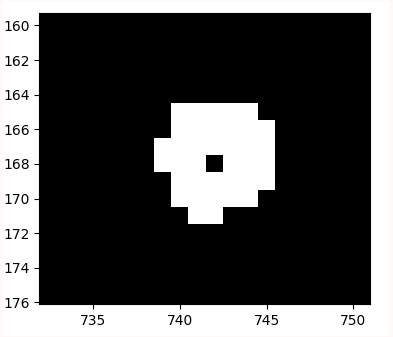
\includegraphics[scale=1.50]{images/circle_object.png}
        \label{img:circle_objects}
        \caption{Sobel circles around objects}
    \end{center}
\end{figure}

Figure 3.5 shows example of correctly identified object.

\begin{figure}[H]
    \begin{center}
        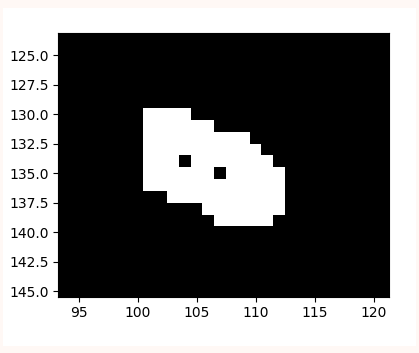
\includegraphics[scale=1.50]{images/joined_objects.png}
        \label{img:joined_objects}
        \caption{Joined sobel circles}
    \end{center}
\end{figure}

Figure 3.6 shows one of the challenges of this solution and that is the fact that some objects are joined together because of the 2D projection.
Cases like this one are hard to separate and if they are overlapping even more, they are inseparable.
We could imagine extracting this double object together but this object would be impossible to use in next stage of segmentation, therefore we consider only objects with circular shape with only one joined empty space in the middle.

\subsection{Second derivative thresholding}
During early stages of implementation, intuitive solution to segmentation was proposed.
After process similar to one described in section 3.3.3, we obtain histogram of the data.
Most of the data is attributed to noise, therefore we can expect spike in the histogram values near the lower edge tracing curve with gaussian-like shape.
Second derivative of this curve therefore first rises, then at the top of the gaussian bell decreases to negative values and the rises again to a positive.
Another way to describe this change is by the shape of the curve in immediate vicinity of the point, it's concavity.
It changes from convex to concave and then convex again.
While higher values are rare, the rest of the curve oscillates around second derivative equal to 0.
We can therefore imagine that segmentation could be performed by finding appropriate thresholding value by finding where the biggest spikes in second derivative are and finding their second local maximum.
This approach works in vast majority of the cases, but proves to be challenging when SNR approaches 1.
The biggest disadvantage of this method is that it does not give us option to fine tune this thresholding value if segmentation detects too many or too little points.

\section{Cluster creation}
After segmentation is done, we are presented with binary bitmap mask marking pixels that passed segmentation with positive value.
We first need to combine these pixels into separate clusters of neighboring pixels.
After every cluster is created as a separate object, we can start analyzing the data.
In the implementation chapter we will explore capabilities of these objects.

\subsection{False detections}

In both approaches to segment the data in this chapter, we set some thresholding value whether it is intensity threshold, or steepness threshold in form of value after combining sobel operators for both dimensions.
All of these perform with good results in segmenting point-like objects.
In the case of streak objects the situation changes.

\begin{figure}[H]
    \begin{center}
        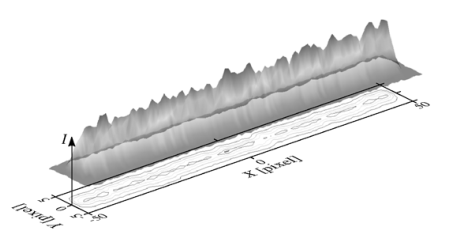
\includegraphics[scale=1.50]{images/streak3d.png}
        \label{img:joined_objects}
        \caption{3D view of streak \cite{kouprianov}}
    \end{center}
\end{figure}

As we can see in Figure 4.5, streaks behaves differently than point-like objects.
Streak object does not have clear maximum as would happen in case of point-like objects.
This fact implies that after segmentation, multiple objects could be detected, all coming from same original streak-object.
This behavior is expected and gives us multiple options how to deal with these false findings.

\begin{itemize}
    \item Ignore all objects within small region over the threshold
    \item Analyze objects after segmentation
    \item Use different segmentation method
\end{itemize}

One solution that would eliminate most of the false positive results is to join neighboring points after segmentation and consider only objects with specific size.
We know the length of the streak from exposure time that can be provided in header of input data from observatory.
This approach would work but brings complications because streaks can be rotated as well as ignoring possibly vast amount objects in cases of lower SNR.\\
\indent
Second option is to consider all the detections but give them some value of validity.
This approach was implemented as it gives option of later interaction with this validity value.
For this purpose we used approach from statistics, skewness and kurtosis. We calculated these statistical metrics along both axis through the peak of each object.
\indent
Last option is to use some other segmentation method that would consider this streak shape from the start, but post-segmentation analysis feels like natural fit for this case with advantage of having the same segmentation for both shapes of objects.

\subsection{Skewness}
Skewness measures the degree of distortion from the symmetrical bell curve \cite{numerical_recipes}.
It measures the lack of symmetry in a distribution.
Skewness can have positive as well as negative values

\begin{itemize}
    \item $skewness < 0$ \\
        tail of distribution is longer on right, median of distribution is lower than it's mode
    \item $skewness = 0$ \\
        distribution is perfectly symmetrical
    \item $skewness > 0$ \\
        tail of distribution is longer on left, median of distribution is higher than it's mode
\end{itemize}

This value is calculated from cross section of object and will be used in another stage of our pipeline to help determine false positive result.
If we would predict object to be valid detection and absolute value of skewness would be high enough, we would conclude that this detection must be false positive.\\
We calculate skewness with formula

$$\frac{1}{n} \sum_{n=1}^{n} [ \frac{x_i - \bar{x}}{\sigma} ]^3$$

        where $x_i$ is intensity of given pixel, $\bar{x}$ is mean value and $\sigma$ is standard deviation

\subsection{Kurtosis}
Kurtosis measures tails of the distribution, it is used to describe extreme values in one tail against the other tail \cite{numerical_recipes}.
It measures outliers of a distribution.

\begin{itemize}
    \item $kurtosis < 0$ \\
        low kurtosis values detect that distribution has light tails, and very little outliers
    \item $kurtosis = 0$ \\
        shape of standard distribution
    \item $kurtosis > 0$ \\
        high kurtosis values detect heavy tails, many outlier
\end{itemize}

We calculate kurtosis with formula
$$\{\frac{1}{n} \sum_{n=1}^{n} [ \frac{x_i - \bar{x}}{\sigma} ]^4\}-3$$

where all the variables are identical to values in section about skewness in this chapter.
Normally, shape of standard deviation has kurtosis value of 3, but it is convenient to have our desired shape with a value of 0 (same as with skewness), therefore we subtract 3 at the end of our formula (Fisher's definition).

\section{Point spread function}

Point spread function (later only PSF) describes response of imaging system to and object being captured by this system.
More specifically, it is a method that describes the way this system distorts the data we observe.\\
This method is being used in many different bodies of science, for example microscopy, lithography.
While in astronomy sources of data are pretty straight forward, having basically circular shapes, most of the distortion present in PSF comes from the atmospheric turbulences.
Our goal with using of this method is to find function that mathematically describes our object of interest.
While stars are basically all the same shape and size, they get distorted by atmospheric turbulences similarly.
This is not the case of space debris and where distribution may vary hugely.
Therefore finding this function gives us all the information we need to decide if object is relevant.
Fitting of function to the data stops dependency upon the original raw image while retaining all the necessary data for further processing in the next steps of our pipeline.

\subsection{2D Gaussian}

In case of point-like objects, 2d version of gaussian provides the closest fit.
We will use version of 2d gaussian with sensitivity to rotation as this proves to be useful while fitting streak-like objects.
In the next chapter we provide another function for streak-like objects, but with rotation, separation of standard diviation in 2 dimensions, 2d gaussian is capable of providing good fit for streak-like objects too.
We use 2d gaussian with this formula

$$ f(x,y) = O + A \exp(-(a(x-x_0)^2 + 2b(x-x_0)(y-y_0) + c(y-y_0)^2)) $$

with a, b and c defined as follows

$$ a = \frac{\cos^2\theta}{2\sigma_x^2} + \frac{\sin^2\theta}{2\sigma_y^2} $$

$$ b = \frac{\sin 2\theta}{4\sigma_x^2} + \frac{\sin 2\theta}{4\sigma_y^2} $$

$$ c = \frac{\sin^2\theta}{2\sigma_x^2} + \frac{\cos^2\theta}{2\sigma_y^2} $$

where

\begin{itemize}
    \item A - amplitude
    \item O - offset
    \item $\theta$ - clockwise rotation
    \item $\sigma_x$ - standard deviation parallel to x axis
    \item $\sigma_y$ - standard deviation parallel to y axis
    \item $x_0$ - position of peak in x axis
    \item $y_0$ - position of peak in y axis
\end{itemize}

This formulation provides all the variation needed to fit any point like object with normalized root mean square(RMS) lower than 0.1.

\begin{figure}[H]
    \begin{center}
        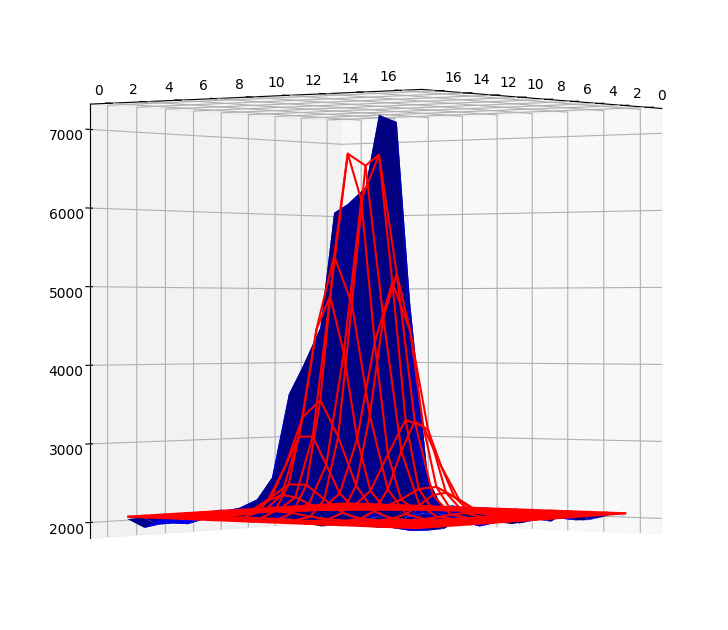
\includegraphics[scale=2.00]{images/gauss_point.png}
        \label{img:gauss_point}
        \caption{Correct gaussian fit to point-like object}
    \end{center}
\end{figure}

The figure 4.6 shows one of the correct fits to the point-like object.
The blue surface plot shows original data, while red wire frame shows values present on the same coordinates according to two-dimensional gaussian with our fitted parameters.
It might look little bit misleading, mostly on the top of the object where peaks do not align, but that is just a relic of the visualisation.
This image contains just 16x16 pixels and visualisation does not interpolate any points between discrete values, just joins them to form a grid.


\begin{figure}[H]
    \begin{center}
        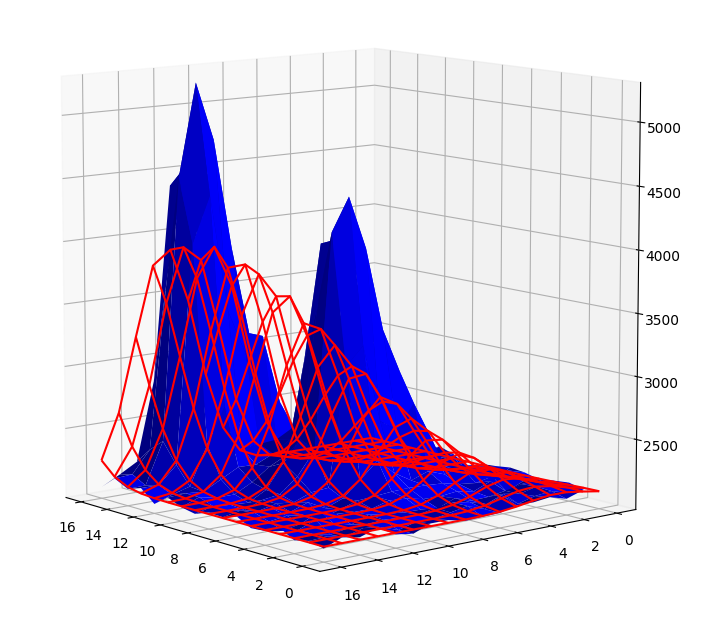
\includegraphics[scale=2.00]{images/gauss_point_bad.png}
        \label{img:gauss_point_bad}
        \caption{Incorrect gaussian fit to point-like object}
    \end{center}
\end{figure}

Figure 4.7 shows one of the issues we are dealing with during fitting, but shows easy way to detect mistakes during segmentation.
As we can observe, we managed to detect two overlapping objects, joining them to a single cluster.
Detections like this cannot be used as some parts of the object are covered by the second one and fit will always be biased.
We need to be able to detect these incorrect segmentations before later stages of pipeline, and this is easy to do at this point.
Part of the data exported contains full width half maximum (FWHM) in both dimensions, and overlapping objects will have much higher FWHM in one dimension even thou we managed to fit even data like this with RMS of 0.1.

\begin{figure}[H]
    \begin{center}
        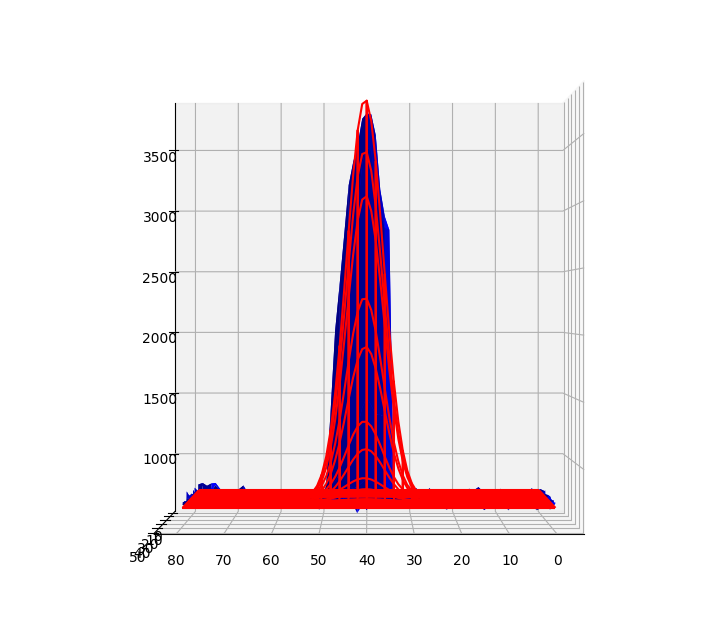
\includegraphics[scale=2.00]{images/gauss_streak.png}
        \label{img:gauss_point_bad}
        \caption{Reasonably good gaussian fit to streak-like object}
    \end{center}
\end{figure}

In some cases even streak-like objects are fitted flawlessly.
It happens mostly in cases of shorter streaks in the dimension of it's tail.
In Figure 4.8 we see one of these cases while in Figure 4.9 we can observe situation that happens in vast majority of cases.

\begin{figure}[H]
    \begin{center}
        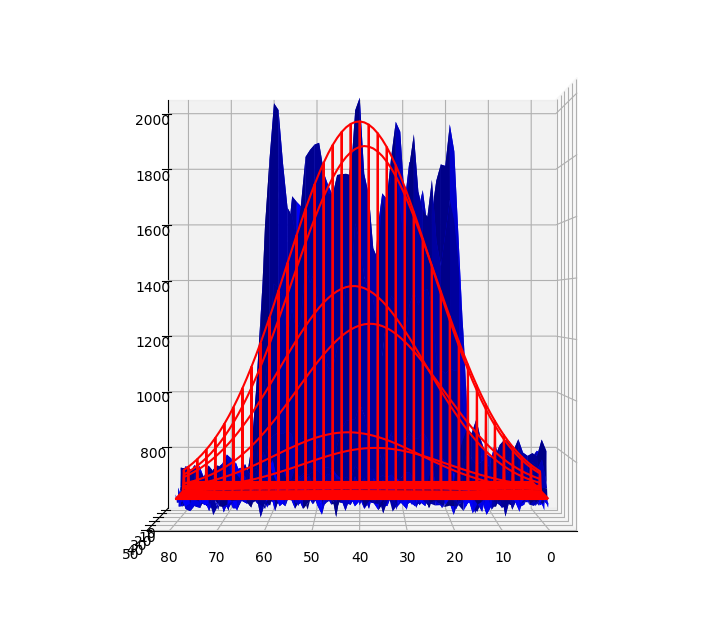
\includegraphics[scale=2.00]{images/gauss_streak_bad.png}
        \label{img:gauss_point_bad}
        \caption{Gaussian fit to streak-like object}
    \end{center}
\end{figure}

Even thou fit is reasonably good according to RMS, shape of gaussian function can never match shape of the data correctly because gaussian does not have that flat top that provides the closest approximation to the streak shape \cite{stovaken}.

\subsection{PSF-Convolution Trail Function}
PSF-Convolution Trail Function provides closer match than 2d gaussian in cases of streak-like objects \cite{veres}.
The reason is that streak-like objects, as seen in Figure 4.9, descend to small intensity values rather quickly at the ends of the trail and contain flat top.
As we will discuss later on, 2d gaussian can still provide reasonably good fit with RMS error lower than 0.1, yet convolution trail function can mimic this shape better.
\\
We approximate the trail as the convolution of an axisymmetric Gaussian PSF moving at a constant rate in direction of rotated (if needed) x axis.
Another models could be used instead of Gaussian such as Lorentz or Moffat but objects we are dealing with most closely resemble gaussian profile.
According to proposed solution, intensity value of any point is equal to

$$f_T(x',y') = b(x',y') + \frac{\phi}{L} \frac{1}{\sqrt{2\pi\sigma^2}} \times \int_{-L/2}^{+L/2} exp\bigg[-\frac{1}{2\sigma^2}{(x'-l)^2 + (y')^2}\bigg] dl$$

where

\begin{itemize}
    \item $\phi$ is the cumulative intensity of a trail
    \item $b(x',y')$ is the value of the background at a point
    \item L is length of the trail
    \item $\sigma$ is standard deviation of our convolved gaussian
\end{itemize}

This trail equation can be enriched by rotation with respect to the $+x$-axis such that
$$x'=(x-x_0)\cos{\theta} - (y-y_0)\sin{\theta}$$
$$y'=(x-x_0)\sin{\theta} + (y-y_0)\cos{\theta}$$

Whole equation, combined with the rotation can be rewritten using error function

$$ \text{erf}(z) = \frac{2}{\sqrt{\pi}} \int_{0}^{z}e^{-t^2} dt$$

yielding the trail equation

$$ f_T(x,y)=b(x,y)+\frac{\phi}{L}\frac{1}{2\sigma \sqrt{2\pi}} \times \text{exp} \bigg[ - \frac{b^2}{2\sigma^2} \bigg] \times \bigg( \text{erf} \bigg[ \frac{a+L/2}{\sigma\sqrt{2}}\bigg] - \text{erf} \bigg[ \frac{a-L/2}{\sigma\sqrt{2}} \bigg] \bigg) $$

where $a$ and $b$ are substitutions
$$ a = (x-x_0)\cos{\theta}+(y-y_0)\sin{\theta} $$
$$ b = (x-x_0)\sin{\theta} + (y-y_0)\cos{\theta} $$

This lengthens initial gaussian estimation in the direction of x-axis yielding streak-like shape with flat top

\begin{figure}[H]
    \begin{center}
        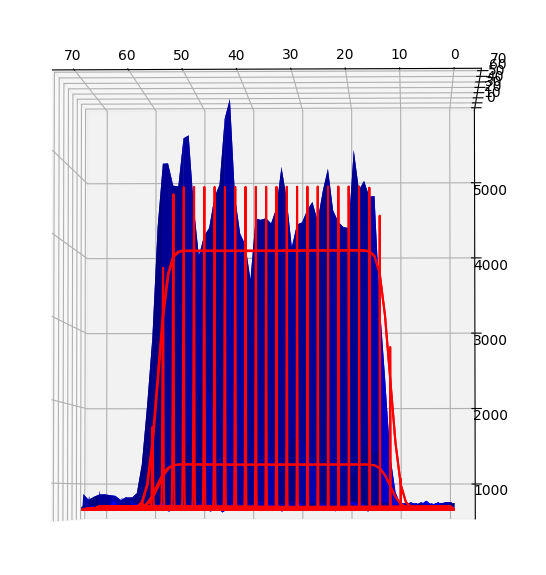
\includegraphics[scale=2.00]{images/veres_front.png}
        \label{img:veres_front}
        \caption{View perpendicular to axis parallel to streak - front view}
    \end{center}
\end{figure}

\begin{figure}[H]
    \begin{center}
        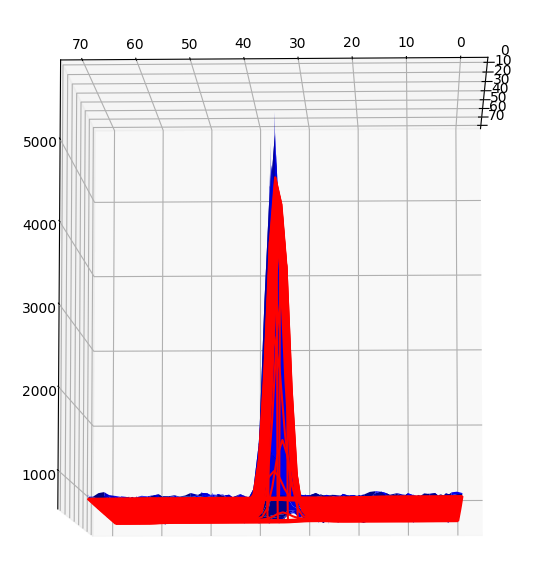
\includegraphics[scale=2.00]{images/veres_side.png}
        \label{img:veres_side}
        \caption{View along axis parallel to streak - side view}
    \end{center}
\end{figure}

While two-dimensional gaussian provides all the necessary information with same precision, except total intensity of a trail, we did not implement fitting of this function.
However, if parameters are provided in the header of FITS file we can nevertheless plot this function and collect total intensity from the data.
During implementation we decided that while gaussian fit is necessary for PSF-Convolution Trail Function and it's fitting iteration performs orders of magnitude faster, we will not be using this function but we will leave it implemented in the codebase for potential future improvement.

\subsection{Function fitting}
Fitting a function to an object is the process where some specified algorithm tries to find parameters to a pre-defined function so that it minimizes the error between said function with it's parameters and the actual data.
We are using least squares approach to minimize this error \cite{watson1967}.
In particular we are minimizing error by applying Lavenberg-Marquardt method \cite{lavmar} for unconstrained problems and Trust Region Reflective method \cite{trf} (TRF) for fitting with bounds.
We calculate moments as initial approximation for the 2d gaussian therefore TRF is mainly used.
This approach basically means that we are trying to minimize the sum of squares between an observed value of real data and the fitted value provided by function with said arguments.
Function usually contains multitude of parameters that are fitted by this approach and produces function with one argument ($f(x)=y$).
This basically means that we are trying to fit curve to a data set.
In our case we are dealing with two-dimensional data in form of image, it's $x$ and $y$ positions and output in form of intensity of pixel $image[y][x]$.
It means that we are fitting curved plane to this three-dimensional space ($f(x,y)=z$).
\\
Finding the perfect fit to a data, apart from some trivial cases, is unrealistic.\\
Whole process of fitting takes two parameters which need to be specified to decide between quality of fit and time spent during computation
\begin{itemize}
    \item maximum number of iterations
    \item tolerated error
\end{itemize}

Command line interface of final solution gives user option to specify these with some preferred default values.

\subsection{Testing}

In this subsection we will compare results of our solution with established astronomical tool.
We are comparing ability of our software to detect position of object's peak with precision of two decimal places.
Data produced in this subsection are produced by script described in Subsection 5.2.8.

\begin{table}[H]
    \centering
\begin{tabular}{|r|r|r|}
\hline
    astrometrica & our solution & euclidean distance\\ \hline
    (1002.29, 685.45) &  (1002.17, 685.47) & 0.1217\\ \hline
    ( 949.31, 889.42) &  ( 949.23, 889.51) & 0.1204\\ \hline
    ( 957.30, 211.97) &  ( 957.32, 211.98) & 0.0224\\ \hline
    ( 952.27, 916.28) &  ( 952.10, 916.40) & 0.2080\\ \hline
\end{tabular}
    \caption{Comparison of few randomly selected peak positions between well established astronomical tool (astrometrica) and our solution (3869\_R\_2-013.fit)}
    \label{tab:compare_peaks}
\end{table}

In Table 4.1 we can observe differences in some randomly selected points from real data collected from AGO showing that our fitting solution finds peaks within distance of 0.2 pixels from the astrometrica's findings.


\begin{table}[H]
    \centering
\begin{tabular}{|l|l|l|l|}
\hline
    file & x & y & average \\ \hline
    3869\_R\_2-013.fit & 0.2291 & 0.2306 & 0.2298 \\ \hline
    3869\_R\_2-013\_gen.fit & 0.0174 & 0.0193 & 0.0183 \\ \hline
    96052C\_1\_R-0003\_d.fit & 0.237 & 0.1651 & 0.201 \\ \hline
    96052C\_1\_R-0003\_gen.fit & 0.0765 & 0.0815 & 0.079 \\ \hline
    E10012B\_2\_R-0003\_d.fit & 0.25 & 0.2127 & 0.2314 \\ \hline
\end{tabular}
    \caption{Distances between astrometrica's detections and our detections. Compared each coordinate separately as well as their average.}
    \label{tab:compare_peaks}
\end{table}

In Table 4.2 we show differences between peaks of all detected objects by astrometrica and compared them to peaks detected by our solution.
Tests are performed on real data as well as data produced by replacing all the objects by synthetic ones.
We can observe that detections are at most 0.2 pixels apart and this difference even minimizes when synthetic objects are detected.



\chapter{Design and implementation}

\section{Design}

The application runs in a console with fully functional Command-line interface (CLI) but provides option to use a graphical user interface (GUI) as well.
GUI is unidirectional meaning that we can see intermediate products when certain flags are specified, but we cannot alter latter stages of the process though this interface.
Reason why we do not implement fully functional GUI is that this code will ultimately be used as a part of the pipeline where it will be ran by another script and has to function with minimal human interaction.
That being said, seeing intermediate products during development as well as after development to observe some edge cases is useful.

\section{Deployment}

The application will be deployed on Supermicro SuperServer 7048R-TR computer running Linux operating system with following specifications

\begin{itemize}
    \item Intel® Xeon® E5-2640 v4
    \item Intel® Turbo Boost Technology, hyper-threading
    \item 32GB of ECC DDR4 SDRAM 72-bit system memory
    \item 400GB SSD system disk
    \item 4TB SATA 3.0 HDD in RAID1 additional data
    \item 920W power supply
    \item additional slots for CPU, RAM and GPUs for future upgrade
\end{itemize}

The language of implementation chosen makes our solution platform independent therefore it is able to run on almost any hardware or software.

\section{Language of the implementation}

Language chosen for the implementation is python.
Python as one of newer higher level languages has reputation of being slow and bringing unnecessary overhead to a task.
All of these concerns do have a point and performing computationally heavy task with pure python loops would be unwise.
That being said, python developers over the years assembled vast collection of modules that provide functionality implemented in different, faster language while providing interface with python code that is easier to read with less lines of code.
As a result, python takes a role of a glue between more efficient code, while maintaining readability for less experienced coders as well as programming novices.
This lead to many scientists adopting python to create more modules with orientation to specific scientific disciplines.
In implementation of this thesis we used some of these modules to provide efficient computation on arguably large two-dimensional arrays.\\
With efficiency in mind we are using following packages
\begin{itemize}
    \item numpy
    \item scipy
    \item astropy
    \item matplotlib
    \item plotly
\end{itemize}

% \subsection{numpy}
% Numpy is the essential open-source package for performing calculations with n-dimensional arrays in python.
% It gives python program capability to specify data types for our n-dimensional arrays as well as performing complex mathematical operations on these data structures.
% Most of the computation made by these mathematical operations are off-loaded to more computationally efficient code written in Fortran and C programming languages.

% \subsection{scipy}
% Scipy is another open-source package for scientific computing.
% It is built on top of numpy, being fully compatible with numpy's n-dimensional arrays.
% This package accumulated over the years vast pool of algorithms used in plentitude of scientific disciplines.
% In this thesis we are using this package for it's superior least square fitting functions, integration, statistical functions, convolution operations and some more general functions that are too specific to be included in numpy package.

% \subsection{astropy}
% Python due to it's increasingly widespread use in astronomy accumulated multiple packages designed to be used in astronomy.
% Astropy is a collection of said software packages created to unify effort of astronomists around the world.
% For purpose of this thesis we are using this package for loading of data from files with .fit/.fits extensions.
% Astropy offers some predefined models for object fitting, but while these are abstraction above numpy and scipy, we are loosing some functionality that these packages provide as a price for more concise code.
% We implemented these solutions but we do not use them in the pipeline because we are missing some flexibility during fitting.

% \subsection{matplotlib}
% Matplotlib is package providing python bindings for plotting of the data.
% Package supports two-dimensional data as well as three-dimensional data visualisation.
% For the purpose of the pipeline we don't need to plot the data, but this package was heavily used during implementation and it gives us ability to observe what algorithm did to the data after segmentation as well as fitting.
% Command line interface of the final solution offers multiple optional arguments to provide this visual overview during choice of parameters.
% \\
% \subsection{plotly}
% While matplotlib has the ability to plot three-dimensional data, it does not perform smoothly as it was not originally made with this use-case in mind.
% Data can always be exported to a file with .fit extension and visualised in another program, but to avoid breaking workflow while exporting data we added also this javascript visualisation alternative.

\section{Objects and modules}

Implementation consists of both objects as well as scripts with single concise functionality.
Entire process is being run by command line interface implemented in the main script.

\subsection{Project structure}
Project is separated into one folder with one sub-folder containing data from our observatory as well as some synthetic images used mostly during background estimation.
Project structure\\

\begin{itemize}
    \item data/
    \item background\_extraction\_cli.py % done
    \item psf\_segmentation\_cli.py
    \item PointCluster.py
    \item hist\_threshold.py % done
    \item utils.py % done
    \item plotting.py % done
    \item testing\_parser.py
    \item decorators.py % done
\end{itemize}

\subsection{background\_extraction\_cli.py}

For the purpose of our processing pipeline, background estimation and extraction is implemented in a separate module.
Entirety of the script is wrapped in a separate command line interface focused on loading data, performing extraction and outputting extracted background to the file.
The file contains multiple functions as well as a pythonic main function containing command line parser.

\begin{center}
    \begin{tabular}  { | p{0.5\linewidth} | p{0.5\linewidth} | }
        \hline
        Method and arguments & Definition \\
        \hline
        convolve(image, kernel\_size, kernel\_type) & method responsible for convolving the image\\
        \hline
        gauss\_kernel(size, sigma) & creates gaussian kernel according to specified parameters \\
        \hline
        image\_preprocess(image) & performs image preprocessing on the image as specified in subsection 3.2.1 \\
        \hline
        sigma\_clipper(image, num\_tiles\_width, num\_tiles\_height, iterations) & fetches sigma clipping result and box-blurs the result (if tiling parameters specified, runs on tiles and joins them) \\
        \hline
        perform\_sigma\_clipping(image, iterations) & starts sigma clipping process with multiple iterations \\
        \hline
        fix\_sizes(image1,image2) & makes both images equal size according the to size of the smaller one, if preprocessing changes size with convolution process \\
        \hline
        show\_hist(image) & creates histogram and shows it with matplotlib \\
        \hline
    \end{tabular}
\end{center}

If file is ran directly, it executes it's pythonic main function and runs command line interface parser with following arguments

\begin{center}
    \begin{tabular}  { | p{0.5\linewidth} | p{0.5\linewidth} | }
        \hline
        Argument name & Definition \\
        \hline
        file & mandatory argument, specifies target of sigma clipper \\
        \hline
        -i & specifies number of iterations, with default number of 5 \\
        \hline
        -o & name of output file (if not specified, original file with postfix \_bg is used)\\
        \hline
        -a & boolean argument, notifies the script that file is in absolute path format and result should be placed in the same directory \\
        \hline
    \end{tabular}
\end{center}

\subsection{psf\_segmentation\_cli.py}

This file is the core file that is being ran to produce results.
The file contains separate command line interface with following arguments that user or automated pipeline interacts with.

\begin{center}
    \begin{tabular}  { | p{0.5\linewidth} | p{0.5\linewidth} | }
        \hline
        Argument name & Definition \\
        \hline
        file & target file \\
        \hline
        -f & function used for object fitting \\
        \hline
        -o & file to output data into \\
        \hline
        -s & segmentation method used \\
        \hline
        -sq & width, height of square we fit around the peak of the cluster \\
        \hline
        --sigma\_threshold & number of sigma removed to the right from center of gaussian fitted to histogram \\
        \hline
        --sobel\_threshold & thresholding value for sobel operator segmentation \\
        \hline
        --background\_iterations & number of iterations during sigma clipping \\
        \hline
        --show\_segmentation & show the result of segmentation \\
        \hline
        --show\_object\_fit & show the result of each object fitting \\
        \hline
        --show\_object\_fit\_separate & show the result of each object fitting, but firstly original data, then fit \\
        \hline
        --show\_fit\_threshold & show the result of thresholding fit \\
        \hline
        --show\_3d & show image in 3d before segmentation \\
        \hline
    \end{tabular}
\end{center}

and contains multiple methods used to create PointClusters and start their fitting process

\begin{center}
    \begin{tabular}  { | p{0.5\linewidth} | p{0.5\linewidth} | }
        \hline
        Method and arguments & Definition \\
        \hline
        threshold\_extract\_clusters(image, sigma\_threshold, show\_segmentation, show\_fit\_threshold) & performs cluster creation with fit thresholding as specified in Section 4.2.1 \\
        \hline
        sobel\_extract\_clusters(image, show\_segmentation, threshold) & performs cluster creation with sobel operator as specified in Section 4.2.2 \\
        \hline
        join\_neighbor\_points\_mask(mask) & iteratively joins neighboring points together \\
        \hline
    \end{tabular}
\end{center}

The module also contains pythonic main function that starts command line argument parser.

\subsection{PointCluster.py}

This object contains all the information about single object, it performs fit on itself and returns result about the fit.

\begin{center}
    \begin{tabular}  { | p{0.5\linewidth} | p{0.5\linewidth} | }
        \hline
        Method and arguments & Definition \\
        \hline
        add\_background\_data( self, background\_data ) & adds PointCluster reference to background data \\
        \hline
        add\_header\_data( self, header\_data ) & adds PointCluster reference to header data \\
        \hline
        fit\_curve(self, function, square\_size) & performs fitting with specified function with given size of the frame \\
        \hline
        fill\_to\_square(self, square\_width, square\_height, center) & creates smaller image we perform fitting on according to a size (around peak or specified center) \\
        \hline
        gaussian\_2d(self, data\_tuple, amplitude, xo, yo, sigma\_x, sigma\_y, theta, offset) & returns two-dimensional array with values equal to gauss with specified parameters \\
        \hline
        veres(self, data\_tuple, x0, y0, width, length, rotation, total\_flux) & returns two-dimensional array with values equal to PSF-Convolution function with specified parameters \\
        \hline
        moments(self, data) & returns estimation of height, x, y, width\_x, width\_y calculated from moments \\
        \hline
        output\_data(self) & returns string representation of the PointCluster, one line of the output \\
        \hline
    \end{tabular}
\end{center}


\subsection{plotting.py}

Plotting module in this case joins all the plotting functionality we needed during implementation as well as during usage.
This module has capability to plot two-dimensional data as a grid with colored squares ranging from black for lowest value to white for maximal value.
If data provided is wrapped in the regular python list, it creates subplot for each.
\\
More useful than two-dimensional plotting for our use case is three-dimensional plotting.
For this very purpose we are using the same module as for two-dimensional plotting, namely matplotlib.
Data is visualised as a surface plot with option to provide additional data arrays which we visualise as red wire frame plot.
This proves to be very useful when comparing actual data with data predicted by our fitted model.
Matplotlib was not created with 3D capabilities in mind and therefore suffers in terms of higher latency on arrays of size 1024x1024.
If smooth visualisation is desired, we provide another plotting alternative, javascript based visualisation in web browser called plotly.


\begin{center}
    \begin{tabular}  { | p{0.5\linewidth} | p{0.5\linewidth} | }
        \hline
        Argument name & Definition \\
        \hline
        show\_data(data,name) & plots two-dimensional data or subplots if list given instead \\
        \hline
        show\_3d\_data(data, label, method, secondary\_data, color) & plots three-dimensional data with given method of plotting, label and color (if secondary\_data is specified, plots it with red wire frame) \\
        \hline
    \end{tabular}
\end{center}

\subsection{utils.py}

This little module contains simple methods with constrained functionality, therefore it makes sense to have them in separate module.

\begin{center}
    \begin{tabular}  { | p{0.5\linewidth} | p{0.5\linewidth} | }
        \hline
        Method and arguments & Definition \\
        \hline
        normalize(data) & performs normalization on the data and returns this normalized data \\
        \hline
        rms(data,predicted) & returns root mean square between data and predicted data \\
        \hline
        psnr(data,bg\_median, noise\_dispersion) & returns peak signal to noise ratio of the data \\
        \hline
        neighbor\_check(first\_point, second\_point) & checks if two points are in their immediate vicity \\
        \hline
        progressBar(value, total, bar\_length) & creates progress bar showing object fitting progress \\
        \hline
    \end{tabular}
\end{center}

\subsection{hist\_threshold.py}

The default option of segmentation (as defined in section 4.2.1) performs segmentation by fitting gaussian function to the histogram of the data.
This module contains all the logic needed to create histogram, fit function to it and return thresholding value based on number of sigma specified by command line argument.

\begin{center}
    \begin{tabular}  { | p{0.5\linewidth} | p{0.5\linewidth} | }
        \hline
        Method and arguments & Definition \\
        \hline
        gaussian(x, amp, cen, wid) & returns value of gaussian at given point with specified parameters \\
        \hline
        histogram\_threshold(image,show, threshold\_sigma) & returns value of threshold specified number of sigma to the right from peak of fitted gaussian (plots fit if show=True) \\
        \hline
    \end{tabular}
\end{center}

\subsection{testing\_parser.py}

For purpose of this thesis we compared results made by our solution and compared them to a existing solution from well established astronomical software.
This module parses the results from our output and compares them to a .cat file from existing solution in order to compare them.

\subsection{decorators.py}

Decorators are one of the very useful feature of python that minimizes amount of lines of coded needed.
These functions are basically functions that can wrap another function and run it with additional functionality before or after.
This proves to be very useful in repetitive task such as logging or timing.
The reason behind these functions is that if we get too many objects and try to fit them with big precision, it takes a lot of time.
It is important to give a user some sort of feedback to decide if he wants to wait or terminate the process.

\begin{center}
    \begin{tabular}  { | p{0.5\linewidth} | p{0.5\linewidth} | }
        \hline
        Method and arguments & Definition \\
        \hline
        time\_function & calculates elapsed time of function run and logs it to standard output\\
        \hline
        print\_function(name) & notifies user of currently ran function \\
        \hline
    \end{tabular}
\end{center}

\section{Output form}

The form of output has to contain all the information necessary but apart from that it can have arbitrary form as long as it is documented properly for next stage of the pipeline.

\begin{figure}[H]
    \begin{center}
        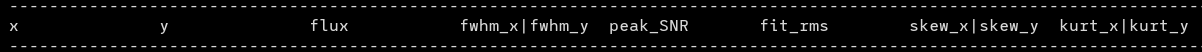
\includegraphics[scale=1.50]{images/output_form.png}
        \label{img:output_form}
        \caption{Header of our output}
    \end{center}
\end{figure}

Output file does not have any specified extension and contains plain text.
First three lines contain two separators and names of columns each with width of 15 characters.
Meaning of each column is as follows

\begin{itemize}
    \item x - x coordinate of peak of the function fitted to the object
    \item y - y coordinate of peak of the function fitted to the object
    \item flux - total intensity of all pixels in the object
    \item fwhm\_x|fwhm\_y - "full width at half maximum" separated into two values, one per each axis with symbol "|" to separate them
    \item peak\_SNR - PSNR as defined in Section 4.1
    \item fit\_rms - normalized root mean square of our fit as compared to real data
    \item skew\_x|skew\_y - skewness of the object in the middle along specified axis separated by symbol "|"
    \item kurt\_x|kurt\_y - kurtosis of the object in the middle along specified axis separated by symbol "|"
\end{itemize}

Each following line then contains one separate object.


\chapter{Conclusion}

In this thesis we have showed the urgency and need for detecting of orbital objects and summarised the knowledge concerning space debris.
We have scrutinized relevant literature regarding space debris, background estimation and extraction as well as object detection.\\
Firstly we reviewed known techniques used in background estimation, compared them, implemented the most suitable one for our pipeline and described our results in Chapter 3.
In Chapter 4 we reviewed multiple approaches in segmentation, proposed some alterations and also implemented the most fitting approach.
We also described process behind combining the data coming from raw image into relevant data structure as well as showed possible ways to detect incorrect detections.
Then we described process of fitting two-dimensional functions to the objects in order to describe objects mathematically and showed possible improvement in trail objects that will be improved on in the future.
At last we tested results in comparison to already existent solution and commented the difference.
In the last part we thoroughly described all the modules and objects defined in the project so that future work can be done without any ambiguities.\\
This solution will be implemented at the Astronomical and geophysical observatory in Modra on server described in Section 5.2 where it will be connected to the rest of the pipeline and tested on the real data.

\backmatter

\bibliographystyle{alpha}
\bibliography{references}

\listoffigures

\end{document}
